% Using the memoir class.
\documentclass[a4paper,12pt,oneside,openany]{memoir}

% Packages
\usepackage[T1]{fontenc}
\usepackage[utf8]{inputenc}
\usepackage[british]{babel}
\usepackage[style=ieee]{biblatex}
\usepackage{lmodern}
\usepackage{microtype}
\usepackage{soul}
\usepackage{amsmath}
\usepackage{xfrac}
\usepackage{graphicx}
\usepackage{svg}
\usepackage{xcolor}
\usepackage{minted}
\usepackage{siunitx}
\usepackage[style=british]{csquotes}
\usepackage{wrapfig}
\usepackage{tabularray}
\usepackage[linesnumbered,vlined,algoruled]{algorithm2e}
\usepackage{pgfplots}
\usepackage{tikz}
\usepackage{hyperref}
\usepackage[all]{hypcap}
\usepackage[nameinlink]{cleveref}

% Bibliography
\addbibresource{references.bib}
% Biblatex doesn't know about artwork type, so treat as misc.
\DeclareBibliographyAlias{artwork}{misc}

% Formating
\DoubleSpacing
\chapterstyle{bianchi}
\setlrmarginsandblock{2.5cm}{2.5cm}{*}
\setulmarginsandblock{2.5cm}{*}{1}
\setlength{\beforechapskip}{-2cm}
\newlength{\drop}
\captionnamefont{\small}
\captiontitlefont{\small}
\SetAlCapSkip{1em}
\setlength{\interspacetitleruled}{6pt}
\checkandfixthelayout

% Setup
\graphicspath{ {./images/} }
\hypersetup{hidelinks}
\UseTblrLibrary{booktabs}
\usetikzlibrary{tikzmark}
\MakeOuterQuote{"}

\pgfplotsset{width=10cm,compat=1.9}
\usepgfplotslibrary{external}
\tikzexternalize

\crefname{algocf}{alg.}{algs.}
\Crefname{algocf}{Algorithm}{Algorithms}
\PrintSemicolon

% Macros
\newcommand*\mkup[2]{\pdfmarkupcomment[color=yellow]{#1}{#2}}
\newcommand*\refandname[1]{\Cref{#1}: \nameref{#1}}
\newcommand*\incexc[2]{\([#1,#2)\)}
\newcommand*\BitOr{\mathbin{|}}
\newcommand*\ShiftLeft{\ll}
\definecolor{LightGrey}{gray}{0.9}
\SetKw{KwForIn}{in}
\SetKw{KwDoesNotContain}{does not contain}

\makeatletter
\newcommand\semiLarge{\@setfontsize\semiLarge{13.15}{15.18}}
\makeatother

% Patches
\makeatletter
\let\original@algocf@latexcaption\algocf@latexcaption
\long\def\algocf@latexcaption#1[#2]{%
  \@ifundefined{NR@gettitle}{%
    \def\@currentlabelname{#2}%
  }{%
    \NR@gettitle{#2}%
  }%
  \original@algocf@latexcaption{#1}[{#2}]%
}
\makeatother

% Main document
\begin{document}

% Use roman numbering for frontmatter.
\frontmatter
\pagenumbering{roman}

% Title page.
\begin{titlingpage}
    \drop=0.1\textheight
    \vspace*{\drop}
    \centering
    {\LARGE MONASH UNIVERSITY | ARUP}\\[2\baselineskip]
    {
    \LARGE\sffamily 
    TITLE NAME YAY\\TITLE LINE 2
    }\par
    \vfill
    {\LARGE CHALLENGE REPORT}\par
    \vspace{\drop}
    {
        \Large October 2024 \\
        \par
        \large Bachelor of Science Advanced, Global Challenges (Honours) \\
        \large Faculty of Science, Monash University \\
        \large Supervisor: Michael Byrne \\
    }\par
    \vfill
    {\large\bfseries Ben Sutherland | 30380251}\par
    {\large\bfseries Katie Barnshaw | 31442420}\par
    {\large\bfseries Lauren Tran | 32511612}\par
    \vspace*{\drop}
\end{titlingpage}


% Use single spacing for TOC, LOF and LOT
\SingleSpacing

\tableofcontents*

\vspace{2.5cm}
\listoffigures
\vspace{1.5cm}
\listoftables

% Use double spacing otherwise. 
\DoubleSpacing

% Acknowledgements.
\chapter{Acknowledgements}
\begin{semiLarge}
\begin{center}
\enquote*{If you put your mind to it, you can accomplish anything.}
\end{center}
\end{semiLarge}


% Executive summary.
\chapter{Executive Summary}
\vspace{-0.5cm}


% Use arabic numbering for main content.
\mainmatter
\pagenumbering{arabic}

\chapter{Introduction}
As transport networks rapidly expand, the accurate simulation of the impacts of prospective transport management policies becomes increasingly critical. The ability to collect and analyse detailed utilisation data is fundamental to understanding how these complex networks behave, now and into the future. For utilisation data to be a key driver of policy decision making, novel modelling methods that are capable of transforming large modern datasets into meaningful insights need to be designed and tested \cite{ghofraniRecentApplicationsBig2018, welchBigDataPublic2019}. 

A primary use-case for these modelling technologies is evaluating the utility of proposed infrastructure projects in the context of precise demand patterns. While many tools exist for modelling road networks and automobile use, these don't commonly include adequate mechanisms for modelling public transport (PT) networks, which require different considerations \cite{cortesMicrosimulationFlexibleTransit2005}. PT-specific predictive modelling tools are needed to accurately assess the impact of changes to network operation, including infrastructure upgrades, timetable updates or fare policy changes.

This paper presents  "Who's on Board?" (WoB), a novel rail service demand model designed to transform large datasets collected from smart-card-based PT networks into meaningful service-level utilisation data. The WoB reference application with graphical user interface (GUI) and full source code are available on GitHub \cite{bensutherlandWhosBoardRail2024}.

To illustrate the potential uses for WoB the city of Melbourne in Australia is used as case study. Using data from Melbourne's smart-card system, Myki, the crowding, utilisation and transfer characteristics of Melbourne's metropolitan rail network are visualised and further analysed. 

\section{Transport Modelling}
Transport modelling allows new projects to be tested virtually, lowering the possibility of costly mistakes with real infrastructure. The general purpose of modelling is to represent a real world system to better understand that system. More specifically, a model can be used to analyse both existing and proposed systems in real or hypothetical scenarios. 

For transport service demand modelling, the purpose is to understand the interactions between service demand and supply provisioning, beyond what can be observed from raw data alone. Modelling demand at the individual vehicle level creates a far more detailed picture than using overall network capacity and averaged passenger entries as metrics of supply and demand. the ten or hundreds of billions of dollars, a "try besfore you buy" approach becomes increasingly crucial \cite[p.~12]{victorianparliamentarybudgetofficeSuburbanRailLoop2024}.

\subsection{Transport Modelling in Melbourne}
The city of Melbourne in Australia was used as a case study rail network to test the WoB model. Melbourne's public transport system collects detailed patronage data, including both boardings and alightings data and origin-destination data, and has a digitised timetable available in a common format, making it easier to model. These two aspects are common for many public transport systems worldwide, enabling this case study to function as a generalisable example for application of the WoB model. 

\subsection{Mode choice}
When examining general transport networks, there are many transport modes to consider. Automobile use makes up the vast majority of transport, due to the significant amount of investment in road infrastructure globally \cite{minerCarHarmGlobal2024, prieto-curielABCMobility2024}. Commuter data can be considered representative in the absence of data that provides better coverage to discuss mode share. For example, the 2021 Australian census found that in Victoria 85.9\% of commuters travel by car to work every day \cite{australianbureauofstatisticsCensusPopulationHousing2021}. Active and public transport are less commonly used, with trains used by 4.6\% of commuters daily, buses and trams together used by 2.4\%, cycling 1.1\% and walking 3.7\%. As the share of road transport increases, the negative consequences of car use, such as the health impacts of air and noise pollution, sedentary lifestyles, and the climate impacts of emissions will also intensify \cite{frankPathwaysBuiltEnvironment2019, macleodCommutingWorkPostpandemic2022}. Therefore without accessible and appealing public transport these trends will continue \cite{currieAlarmingTrendsGrowth2018, minerCarHarmGlobal2024}. As such, WoB focuses on modelling PT with the aim of improving PT outcomes.

The WoB model runs on a generic timetabled network and therefore, in theory, can model any public transport mode, or connected combination of modes. However, to receive an accurate output, the input data must also be robust. Because of the accessibility and quality of the case study rail data, WoB has been tuned to model rail networks, thus rail modelling is the focus of this research. 

\section{Scope}
\subsubsection{Aim}
To develop a general model for assigning passenger trips from origin-destination data to a rail transport network layout and timetable, producing meaningful service-level utilisation data. 

\subsubsection{Objectives}
\begin{SingleSpacing}
\begin{itemize}
    \item Build a service-level model of train utilisation which is fast, accurate and granular. 
    \item Build a simple user interface for the model that is easy to use. 
    \item Describe crowding cost functions for model implementation. 
    \item Showcase potential model use cases through visualisation of Melbourne train utilisation. 
\end{itemize}
\end{SingleSpacing}

\subsubsection{Key Areas of Focus}
Transport modelling is a broad discipline which attempts to address a wide range of use cases and problems. Given the multitude of ways any single problem can be approached and the solution implemented, there is no ultimate model that can be applied in every situation or solve every problem. Since there are always trade-offs or simplifying assumptions that must be made, different modelling software is specialised for different purposes. By comparing these models, a niche was identified where there are use cases and target users that are not accounted for by existing software \cite{horniMultiAgentTransportSimulation2016, adnanAgentbasedSimulationPlatforma, ZenithMultimodalTransport}. 

With a goal to understand PT utilisation, and support a wide range of end users such as engineers, government planners, advocacy groups and the general public, the following model characteristics have been identified as key areas of focus:

\begin{SingleSpacing}
\begin{itemize}
    \item Accessible
    \item Fast
    \item Granular
    \item Accurate
    \item Predictive
\end{itemize}
\end{SingleSpacing}

The majority of existing transport modelling software is intended for corporate or government use and requires a high level of technical knowledge. To engage a wider range of end users, there are no special knowledge requirements to run the model and it is free and openly accessible to anyone. The setup and operation of the model as described in this paper does not require understanding of the underlying implementation. In contrast to many existing modelling software that are expensive and closed source, the WoB model is free to access in its entirety on GitHub \cite{bensutherlandWhosBoardRail2024}.

Another key area of focus was the speed of the model for rapid feedback and iteration times for the end user. This is particularly useful in planning sessions with professionals and members of the public, as faster run times allows more scenarios to be simulated and altered in real time to generate dialogue and discussion around plans \cite{levinsonApplicationsAccess}. Comprehensive industry-focused models with a broad range of applications (including various modes and additional parameters) can be much more resource intensive to run and as a result, much slower.

Although speed can be bought with greater quantities of hardware with higher specifications, to account for end users from the general public, an ideal model should be able to run on most standard home computers, as opposed to specialised server infrastructure. Currently the average computer memory tends to be between 8GB to 16GB, so memory usage within this range without significantly slowed processing would enable people and groups without significant computational resources to access the model \cite{SpecificationsPersonalComputers}. 

Accurate and granular predictive modelling forms the additional components of the key focuses of the model. The ability to model service-level demand provides far greater detail than aggregated patronage counts, allowing more nuanced understanding of transport trends to emerge. Similarly, ensuring the accuracy of the model means the results can be trusted and used to inform decision making. This requires testing and iteration to verify the accuracy of results, which is much more rigorously carried out by proprietary software, compared to open source projects or one-off models. However, the model prioritises simplicity by optimising for a specific use case, instead of attempting to be applicable to more generalised problems. The more complex a system is, the more challenging it is to capture accurately. By focusing on a single mode, the rail network, rail specific modelling techniques can be applied, rather than adapting road-based techniques. This focused approach lays the foundation for future validation and testing of the model. 

\subsection{Target Users}
WoB's target users form a relatively more diverse range than that of large proprietary software, which tend to be aimed at corporations and engineers in particular. 

\subsubsection{Engineers}
The WoB model should be sufficiently accurate such that engineers can use it to inform or support their projects, such as station redevelopment, timetable changes or upgrades to rollingstock. While WoB is not expected to replace current models, it can complement existing tools by providing an additional perspective in transport modelling projects. 

\subsubsection{Government Planners}
Councils and government departments require predictive modelling capabilities to produce project feasibility studies and understand how policies or infrastructure projects could impact PT utilisation. WoB is free and open source allowing it to be easily accessed in the early stages of project planning before more costly modelling methods are required. The speed of the model also enables rapid adaptation and experimentation which may be costly if done through third-party consulting. 

\subsubsection{Political Advocacy and Special Interest Groups}
Many political advocacy and special interest groups do not have significant resources to spend on computing power or access to proprietary modelling software. Access to WoB would benefit these groups, allowing them to quantify the impact of their proposals. This can strengthen their position in advocating for policy changes such as service frequency upgrades if they can demonstrate the potential improvements. 

\subsubsection{General Public}
For the interested general public, the accessibility of WoB also allows these enthusiasts to gain a deeper understanding of how local or global transport networks behave. A built-in option to generate "random" patronage allows users to interact with the model, irrespective of whether they have access to detailed patronage data. 

\section{Outline}
The following chapter (\Cref{chap:Background}) describes the theoretical background of transport modelling in terms of approaches, simulations, and pathfinding algorithms. The technical details of the construction of WoB is presented in \Cref{chap:ModelConstruction}, outlining the high-level algorithm and the requisite sub-problems, before detailing the specific implemented solutions. \Cref{chap:ModelSpec} discusses the crowding cost functions which describe passenger perception of crowding to inform the allocation of demand to services. \Cref{chap:CaseStudy} demonstrates potential applications of WoB through a case study on the Melbourne metropolitan rail network. Finally, \Cref{chap:Conclusion} sets out potential pathways for future research and concluding remarks.



\chapter{Background}
\label{chap:Background}

The PT service demand model presented in this work builds on many existing technical concepts. This section explores the background information required to understand the implementation of WoB. First, \Cref{sec:TransportModelling} unpacks the various ways transport systems are modelled for different purposes, \Cref{sec:Simulations} considers how simulation techniques can be used to analyse complex problems, \Cref{sec: GTFS} details how public transport networks can be represented digitally, and \Cref{sec:pathfindingalgorithms} outlines pathfinding algorithms that are capable of generating journey itineraries that traverse public transport networks.  

\section{Traditional Transport Modelling}
\label{sec:TransportModelling}
Modelling complex transport systems is a very general problem, for which there is no single solution that can be applied without compromise. The overall goal of modelling transport is to enhance the understanding of a network to accurately test and predict scenarios. The more specific problem of "person travel" (as opposed to freight logistics) remains incredibly broad. One of the most generally applicable and widespread techniques is the Four-Step Forecasting Travel Model \cite{mcnallyFourStepModel2007}.

\subsection{Four-Step Travel Model}
The eponymous four steps are shown in \Cref{fig:four_step_model}.
\begin{figure}[ht]
    \centering
    \includesvg[width=0.75\columnwidth]{images/four_step_flow.svg}
        \caption{Flow chart representing the steps of the four step travel model.}
    \label{fig:four_step_model}
\end{figure}

\pagebreak
Trip generation is the process of combining population and land use data and attempting to predict trips that the population takes across that region. For example, commuter trip patterns can be inferred from commercial and residential zoning patterns. The output of this step is sets of origins and destination locations weighted by some probability. 

Trip distribution takes these origins and destinations and pairs them up probabilistically. There are various algorithms for performing this operation, but generally they are informed by the cost to travel between the two points and the activity purpose of the origin and destination.

The mode choice step allocates the mode or modes (including road, rail, bus, walking, cycling, etc) that compose the trip. Usually, this is also represented as a probability distribution of all the trips between the origin and destination.

In the final round, route assignment, the mode choice distributions are applied to the network itself, yielding a description and quantification of which routes and corridors are used by the modelled population.

One of the key aspects of the four-step model is its self-feedback loop. Once the route assignment is complete, the congestion of the network becomes a known property. This means that the four steps can be run again, this time with network congestion influencing trip distribution and mode choice \cite{mcnallyFourStepModel2007}.

However, as general as it appears to be, the four-step technique suffers from poor predictive outcomes when attempting to evaluate the effect of management and control policies, as opposed to expansion policies \cite{mcnallyFourStepModel2007}. While still in use today, the four-step model is generally used as a base architecture, from which many specialising parameters can be applied. A slightly more modern technique, activity-based modelling, was designed as an alternative \cite{mcnallyActivityBasedApproach2007}.

\subsection{Activity-Based Modelling}
An activity-based model is designed around the idea that travel is a means to an end, and that a more holistic approach that seeks to understand the activities that people travel for will provide a more accurate forecast of travel demand. To achieve this, activity-based models make use of insights from different fields, including behavioural psychology, to create a set of activities that people in a population participate in for a given period at a particular place. From there, patterns of behaviour can be translated into sequences of trips, which thus encode the scheduling of the undertaken activities \cite{mcnallyActivityBasedApproach2007}. Additionally, due to this construction, activity-based models can generally yield more detailed results by allowing analysis of trips per activity, rather than per destination.

\subsection{Comparison to WoB}
As an analogy for our model, the first three steps of the four-step model could be seen to be encapsulated by the input data, which is directly derived from the rail smart-card system rather than land use and demographics. As such, the modelled trips fall within a narrower spectrum, describing only a subset of the movements through the network. There is no mode choice decision either, as all trips are rail-based. WoB does not model activities specifically, which requires first generating the activities then deriving the trips. However, like an activity-based model, the model output is very detailed as individual trips are modelled separately rather than in aggregate.

The pursuit of more and more detailed modelling techniques, building upon activity-based models and aided by the continuous exponential increases in computational power over the decades, has lead to the development of simulations as a viable modelling method.

\section{Agent-Based Simulations}
\label{sec:Simulations}
The general technique of simulations involves the modelling of a system by applying the known rules of the system to a virtual, approximate representation of the system. This broad idea can be applied to many systems from many fields, including transport networks. Detailed transport simulations usually involve keeping records of individual decision-making entities, called "agents". These agents have defined behaviour, which constitutes some of the transport system's rules, in addition to the network layout and transport modes \cite{horniMultiAgentTransportSimulation2016}.

Agent-based simulations have the advantage that they work at a smaller detail scale than other methods. Instead of modelling aggregate parameters, like total patronage or network throughput, these simulations track the properties of each individual agent, and therefore can output a record of the behaviour for each agent. As such, emergent behaviours that occur due to the large number of modelled interactions can be studied.

\section{Timetabled Network Representation}
\label{sec: GTFS}
As described above, PT models that make use of simulation-based approaches require a representation of the timetabled network in computer memory. A key resource for working with PT networks is the General Transit Feed Specification (GTFS), a computer-readable format for defining a network layout and scheduled services on a timetable \cite{mobilitydataReferenceGeneralTransit2024}. A GTFS dataset is generally officially published by a management authority (such as Public Transport Victoria) and contains a record of all the stops, stop times, routes, trips and timetables by calendar day. 

Each stop represents either a station or a platform within a station, depending on the dataset. Stop times are a single stop event in which a vehicle arrives and departs a stop. Trips are sequences of stop times, and represent a particular instance of a vehicle moving through the network. Routes are groups of trips categorised by stop sequences (i.e. all trips in a route visit the same stops in the same order, but at different times). Stops encode the user-facing and geographical information about the stops on the network, such as name and location.

For a model to make use of a PT network representation, a specialised pathfinding algorithm is required to calculate specific paths through the network.

\section{Pathfinding Algorithms}
\label{sec:pathfindingalgorithms}
In contrast to a standard graph network, which can use Djikstra's algorithm and variants thereof for pathfinding, the traversal of a PT network requires the use of specialised algorithms that run on a fixed timetable. There are many such algorithms described in the literature, such as Guidebook Routing \cite{bastFlowBasedGuidebookRouting2014} and the Connection Scanning Algorithm \cite{dibbeltIntriguinglySimpleFast2013}, each of which have different features and drawbacks, explored in detail in the semester one research report \cite{benjaminsutherlandSimulatingMelbournesMetropolitan2024}. 

The Round-bAsed Public Transit Optimised Router (RAPTOR) algorithm was chosen for implementation in WoB \cite{dellingRoundBasedPublicTransit2012} for its ability to run on dynamic networks without preprocessing and its optimised runtime speed. For a given departure station and time, RAPTOR determines the minimum arrival time at each stop in the network by traversing each route on the first available trip over the course of a fixed number of rounds. During round zero, for each route that contains the departure stop the first trip that leaves the departure stop after the departure time is found. Starting at the departure stop, the arrival time at each subsequent stop in the trip is updated. After all relevant stops have been updated in this manner, subsequent rounds work similarly, this time using each updated stop in the previous round as the departure stations. Once no more stops are updated, or a fixed number of rounds has elapsed, the journey that arrives at the desired destination earliest is reconstructed and returned. The RAPTOR algorithm can be extended to perform multi-criteria queries, which allows optimising for more than just minimum arrival time. 

\subsection{Implementation in WoB}
WoB implements the RAPTOR algorithm to determine which services are used by a given agent. To model crowding effects, a key innovation of WoB is the use of the multi-criteria extension to optimise for both earliest arrival time and lowest crowding cost. 


\chapter{Model Construction}
\label{chap:ModelConstruction}

\section{Preliminaries}
The high-level purpose of the train utilisation model is to calculate granular service demand on a particular timetable based on origin-destination data.

% More stuff in here about input and output? Different to thesis by including journey output?

\subsection{High-level Approach}
The design of the model uses an iterative replanning structure to converge on a stable solution. The high-level algorithm of the simulation consists of the following loop:
% This is taken from verbatum from the original thesis.
\begin{SingleSpacing}
    \begin{enumerate}
        \item Set the "crowding cost" of each transit service in the network to 0.
        \item For each set of agent journeys in the input data, determine the transit services used and record the agents as populating the proportion of any trips they use.
        \item Based on the utilisation, calculate a "crowding cost" associated with the transit services.
        \item Go to step 2, or output results and halt.
    \end{enumerate}
\end{SingleSpacing}

\subsection{Existing Work}
The model is a comprehensive extension of the simulation framework completed in semester 1.

\begin{SingleSpacing}
    \begin{enumerate}
        \item Network layout
        \item Normal pathfinding
        \item Assigning passenger counts
        \item Visualisation
    \end{enumerate}
\end{SingleSpacing}

%\subsection{Implementation Details}
%The model was written in Rust, due to its focus on speed and reliability, as well as an ergonomic package ecosystem.

\subsection{Extension to Full Model}
To extend the framework to the full model, the following features were added.
\begin{SingleSpacing}
    \begin{enumerate}
        \item Multi-criteria pathfinding 
        \item Crowding cost functions 
        \item Iterative replanning
        \item OD Data import
        \item User interface
    \end{enumerate}
\end{SingleSpacing}

The various crowding cost functions used by the model are discussed in \Cref{chap:ModelSpec}.
Additionally, the performance of the model is investigated in \Cref{sec:Performance}

\section{Multi-Criteria Pathfinding}
A core component of the replanning algorithm is determining routes for agents based on more than just earliest arrival time. Agents must be able to change their routes based on the crowding of the services. 

This technique is called "multi-criteria pathfinding", where an additional cost is taken into account when determining routes. More precisely, the multi-criteria problem asks for a full Pareto-set of journeys leaving a given origin stop no earlier than a given departure time \cite{dellingRoundBasedPublicTransit2012}. 

% TODO: Move to background? It is most relevent to this section.
A Pareto-set is a set in which each element does not dominate any other - i.e., a tradeoff must be made to choose any over any other. A solution dominates another solution if it is strictly better in at least one criterion \cite{bergerAcceleratingTimeDependentMultiCriteria2009}.

% TODO: more accurately, it's an inverse utility function? Because the utility is currently minimised.
As such, the multi-criteria version of the pathfinding algorithm returns a set of different journeys, each with a different associated arrival time and crowding cost. A utility function is applied to each journey to determine which journey a particular agent will take.

The fundamental different between single and multi-criteria algorithm designs is a matter of bookkeeping. During a single-criteria run, only the earliest arrival at a given stop need be recorded, corresponding to a single journey. However, during a multi-criteria run, at each stop a set of earliest arrival time and crowding cost pairs (called "labels") must be stored, which is considerably more complicated. Instead of a simple assignment to update a stop based on a newly found trip, the new label must be added to the list if it is non-dominated, and then remove any newly dominated labels previously in the set.

The data structure that is generally used for recording these Pareto-optimal sets is a "bag", which is a generic (and fairly mundane) term for a set with specific allowed operations. Most general solutions involve dynamically allocating memory in a resizable array, but because these bag operations are extremely frequent during pathfinding they must be as efficient as possible. We can set an upper bound on the number of stored journeys, which discards labels based on some criteria and allows us to statically inline out array. For our purposes, the label with the latest arrival time is discarded because these are generally the least realistic (going to rather extraordinary lengths to avoid crowded services) but this could be replaced with a specific utility calculation.

\section{Iterative Replanning}

% TODO: Halting conditions

\section{Data Import}

\section{User Interface}

\section{Performance}
\label{sec:Performance}

\begin{table}[ht]
    \centering
    \begin{tblr}{
            colspec={lrrrr},
        }
        \toprule
        Algorithm                             & Melbourne & Tokyo & London & Germany \\
        \midrule
        RAPTOR (\unit{\micro\s})              & 51        & 14    & 85     & 84533   \\
        CSA    (\unit{\micro\s})              & 7         & 85    & 247    & 42886   \\
        \(\sfrac{\text{RAPTOR}}{\text{CSA}}\) & 7.29      & 0.165 & 0.344  & 1.97    \\
        \bottomrule
    \end{tblr}
    \caption[Pathfinding benchmarks]{Time to perform one pathfinding query across the network. Taken from the average of 5000 samples on a 4.5GHz core.}
    \label{tab:PathfindingBenchmarks}
\end{table}
\vspace{-0.7cm}



\chapter{Crowding Modelling}
\label{chap:ModelSpec}

\section{Crowding Cost}
\label{sec:crowding_cost}
While increasing PT usage is generally considered a net positive, an equilibrium must be struck between high PT use and the physical constraints that impact perception of service quality. Low crowding may suggest the transport network is underutilised, but as utilisation increases, high crowding may in turn disincentivise people from using PT more frequently \cite{luanPassengerorientedTrafficControl2022}. The timetabled frequency and routes can be adjusted to produce an equilibrium point between these factors that promotes sustainable growth of PT use. WoB enables the investigation of how timetable or network changes may influence the relationship between utilisation and crowding. 

Crowding cost functions define a relationship between the number of people on board a service and a numerical value representing the "perception" or subjective experience of crowdedness. Crowding cost is considered a high priority when people are evaluating the quality of PT and their likelihood to use it, yet it remains a relatively understudied area \cite{mohringOptimizationScaleEconomies1972, turveyOptimalBusFares1975}. In comparison, car congestion has been much more thoroughly studied and is better understood \cite{arnottEconomicsTrafficCongestion1994, johanssonOptimalRoadpricingSimultaneous1997}. One of the reasons for this disparity is the difficulty in conclusively defining and measuring crowding costs \cite{qinInvestigatingInVehicleCrowding2014}. Crowding cost can be interpreted in different ways, such as the utility of avoiding crowding, or a multiplier to perceived travel time. There are also a multitude of ways to quantify crowding, such as load factors and probability of a seat being available \cite{douglasEstimatingPassengerCost2006, yapCrowdingValuationUrban2020}.

There are many studies highlighting the impact of crowding, as it affects service quality and satisfaction \cite{luanPassengerorientedTrafficControl2022}. Crowded services increase anxiety and stress, largely due to physical proximity, the possibility of being late to work and personal safety risks \cite{haywoodCrowdingPublicTransport2017, chengExploringPassengerAnxiety2010, evansCrowdingPersonalSpace2007, coxRailPassengerCrowding2006}.
Beyond the personal implications, crowding also impacts service timeliness, as high passenger density can make it difficult for others to board or alight, elongating station dwell times, and impacting operating speed and travel time reliability \cite{tirachiniCrowdingPublicTransport2013}. The ideal combination of frequency, vehicle capacity, and fare cost can also be influenced by crowding levels. Therefore, the ability to account for crowding in PT modelling is particularly useful for broad applications in transport planning. 

While crowding cost and the related functions are generalised and can be applied in any context, specific choices have been made in this project to tailor the model for use in Melbourne. As a result, this is not an extensive or exhaustive overview of crowding cost functions as it is intended to form the basis for informing the initial implementation of crowding in the model. 

Choosing a specific crowding cost function is highly dependent on the geographical and social context in which the project is grounded and its overall aims. Other factors such as route options and service frequency can also influence perceptions of crowding. There is no single function that is superior in all cases. Since crowding cost is a numerical measurement of passengers' subjective perspective of the costs associated with crowded services, it can vary significantly between demographics. Ideally, the functions would be calibrated through discrete choice modelling on survey data (stated preference analysis) or analysis of travel patterns (revealed preference) collected from passengers \cite{yapCrowdingValuationUrban2020, tirachiniValuationSittingStanding2016, yapPublicTransportCrowding2023, celebiMeasuringCrowdingrelatedComfort2020}. However, undertaking research to empirically determine crowding costs was outside the scope of this project, which focuses on the model construction, as opposed to attempting to develop a rigorous understanding of crowding and its perception in Melbourne. However, including crowding in the model extends the modelling capabilities, allowing it to be used in more complex cases and elucidate more nuanced characteristics of travel behaviour. A general overview of the relevant functions and their feature was prioritised so that these functions could be implemented in the model. The parameters can then be further calibrated by end users if necessary. 

There are various additional types of crowding associated with transport, but this model focuses specifically on in-vehicle crowding, defined as the number of people on train services. Other forms of crowding, such as station and platform crowding, are related but require different modelling capabilities and were therefore excluded from the project scope. 

\section{Crowding Cost Functions}
\label{sec:crowding_cost_functions}
There are general constraints on crowding cost functions that are established across the literature. Representations of crowding cost must be specific to the PT mode as passengers on different modes perceive crowding differently \cite{qinInvestigatingInVehicleCrowding2014}. When taking long distance rail and bus services, a seat is usually expected and having to stand is a significant burden. However, on metropolitan services, people may not expect to have a seat and be willing to stand, and therefore place a lower value on sitting. Buses are also configured differently to trains and are much smaller, further widening the difference in perception of crowding between modes. Since WoB only considers the rail network, only rail-specific crowding cost functions have been implemented. 

A basic property of crowding cost functions is that the crowding cost should increase monotonically with the number of passengers \cite{tianEquilibriumPropertiesMorning2007, qinInvestigatingInVehicleCrowding2014}. The crowding cost should not decrease for any increase in the number of passengers. This aligns with logical expectations as a passenger boarding will never reduce the level of crowding. An additional basic constraint is that the crowding cost should be zero when there are zero people on board, therefore crowding cost functions must pass through the origin \cite{tianEquilibriumPropertiesMorning2007}.  

\subsection{Specific Functions}
\label{subsec:crowding_functions}
This section provides an overview of mathematical crowding cost functions from previous literature accompanied by discussion of their use in the context of this project. The four functions chosen to be implemented in the model can be grouped into two categories: simple mathematical functions and stepped models. For the purposes of visualising the functions, the seated capacity of an X'Trapolis 100 train was used as it is widely run across Melbourne's metropolitan train network \cite{metrotrainsmelbourneWTTNetworkConfiguration2023}. 

\subsubsection{Simple Mathematical Functions}
\label{subsubsec:crowding_simplemath}
This group of simple mathematical functions only require service capacities as parameters. These functions assume a smooth relationship between patronage and crowding cost, and are simple to implement and manipulate for further mathematical analysis. They are also simple to calibrate as they only require the sitting and standing capacities of the trains. 

\smallskip
\noindent{\textbf{Linear}} 


The first function is linear,
\begin{equation}
    \label{eqn:linear}
    y=\frac{1}{S+T} x
\end{equation}
where $y$ is the crowding cost, $x$ is the number of people, $S$ is the seated capacity and $T$ is the standing capacity of each train (\Cref{fig:Crowding_linear}) \cite{klumpenhouwerCostcrowdingModelLight2016}. 

Since the slope of this equation is entirely determined by the sitting and standing capacities, which should be known values, this is very easy to implement. There are no additional coefficients or parameters that need to be calibrated to match empirical measurements of crowding perception. This assumes that crowding cost increases uniformly as the number of passengers increases. The linear equation is best suited for cases where there are few seats, and therefore discomfort due to crowding is more directly linked to the number of people \cite{klumpenhouwerCostcrowdingModelLight2016}. It has also been suggested that a linear equation is not empirically supported by observations, in part because it is deterministic in assigning a constant crowding cost per person and it also assumes crowding is sufficiently smooth \cite{qinInvestigatingVehicleCrowding2014}. 

\begin{figure}[ht]
    \centering
    \begin{tikzpicture}
        \begin{axis}[
                axis lines = left,
                xlabel = Number of people,
                xmin=0,
                ylabel = Crowding cost,
                ymin=0,
                %legend pos=north west,
            ]
        \addplot[smooth,mark=.,purple] table [x=count, y=linear_cost, col sep=comma] {data/Functions/linear_model.csv};
            \addlegendentry{Crowding cost}
        \addplot[domain=0:2000, samples=2, dashed] coordinates {(432, 0) (432, 1.5)};
        \addlegendentry{Seating capacity}
        \addplot[domain=0:2000, samples=2, dotted] coordinates {(1232, 0) (1232, 1.5)};
        \addlegendentry{Total capacity}
        \end{axis}
    \end{tikzpicture}
    \caption[Graph of the linear crowding cost function]{Graph of the linear crowding cost function, $y=\frac{1}{S+T} x$,  where $y$ is the crowding cost, $x$ is the number of people, $S$ is the seated capacity and $T$ is the standing capacity of each train.}
    \label{fig:Crowding_linear}
\end{figure}

\smallskip
\noindent{\textbf{Quadratic}}


The quadratic function accounts for the intuition that crowding cost should increase more slowly when there are fewer passengers on board (\Cref{fig:Crowding_quadratic}). It has the following form, with the same variables as the linear function \cite{klumpenhouwerCostcrowdingModelLight2016}
\begin{equation}
    \label{eqn:quadratic}
    y=\frac{1}{(S+T)^2}x^2.
\end{equation}

In Figure \ref{fig:Crowding_quadratic}, the dotted line at $x=432$ shows the sitting capacity. In the region around this point, the slope of the function begins to increase, indicating crowding cost increasing more rapidly as the number of people increase. However, the behaviour of the function does not change at this point.

\begin{figure}[ht]
    \centering
    \begin{tikzpicture}
        \begin{axis}[
                axis lines = left,
                xlabel = Number of people,
                xmin=0,
                ylabel = Crowding cost,
                ymin=0,
                %legend pos=north west,
            ]
        \addplot[smooth,mark=.,purple] table [x=count, y=quadratic_cost, col sep=comma] {data/Functions/quadratic_model.csv};
            \addlegendentry{Crowding cost}
        \addplot[domain=0:2000, samples=2, dashed] coordinates {(432, 0) (432, 1.5)};
        \addlegendentry{Seating capacity}
        \addplot[domain=0:2000, samples=2, dotted] coordinates {(1232, 0) (1232, 1.5)};
        \addlegendentry{Total capacity}
        \end{axis}
    \end{tikzpicture}
    \caption[Graph of the quadratic crowding cost function]{Graph of the quadratic crowding cost function, $y=\frac{1}{(S+T)^2}x^2$,  where $y$ is the crowding cost, $x$ is the number of people, $S$ is the seated capacity and $T$ is the standing capacity of each train.}
    \label{fig:Crowding_quadratic}
\end{figure}

\subsubsection{Stepped Models}
\label{subsubsec:crowding_stepped}
The second category of functions attempt to build a more nuanced representation of crowding cost by including a discrete step. This primarily addresses the fact that the previous functions do not account for the subjective difference between sitting and standing. The stepped models assume that sitting is preferable to standing and that people automatically assign a higher cost to standing. Both models also assume that when there are seats available, the crowding cost (or perception of crowding) remains the same. 

\smallskip
\noindent{\textbf{One-step}}


The one-step model is given as
\begin{equation}
\label{eqn:onestep}
    y=\alpha_0\frac{S}{x}+\left(1-\frac{S}{x}\right)\alpha_0\left(1+be^{a\left(\sfrac{x}{S}-1\right)}\right)
\end{equation}
where $y$ is the crowding cost, $x$ is the number of passengers, $S$ is the seating capacity, $\alpha_0$ is the cost of sitting. $a$ and $b$ are free parameters which can be modified to adjust the shape of the function \cite{qinInvestigatingInVehicleCrowding2014}. This equation requires that $a>5$ for the correct shape. The one-step model assumes there is a constant cost until all seats are filled, whereafter the crowding cost increases exponentially with the number of passengers. The exponential increase in crowding cost as the number of passengers approaches total capacity performs a similar purpose to the quadratic growth of the previous function. As a train approaches total capacity, it should only be perceived as the superior choice if the alternative service would significantly increase travel time (such as an hour long wait for the next service). 

\begin{figure}[ht]
    \centering
    \begin{tikzpicture}
        \begin{axis}[
                axis lines = left,
                xlabel = Number of people,
                xmin=0,
                ylabel = Crowding cost,
                ymin=0,
                legend pos=north west,
            ]
        \addplot[smooth,mark=.,purple] table [x=count, y=one_step_cost, col sep=comma] {data/Functions/one_step_model.csv};
            \addlegendentry{Crowding cost}
        \addplot[domain=0:2000, samples=2, dashed] coordinates {(432, 0) (432, 1.5)};
        \addlegendentry{Seating capacity}
        \addplot[domain=0:2000, samples=2, dotted] coordinates {(1232, 0) (1232, 1.5)};
        \addlegendentry{Total capacity}
        \end{axis}
    \end{tikzpicture}
    \caption[Graph of one-step crowding cost function]{Graph of the one-step crowding cost function, $y=\alpha_0\frac{S}{x}+\left(1-\frac{S}{x}\right)\alpha_0\left(1+be^{a\left(\sfrac{x}{S}-1\right)}\right)$, where $y$ is the crowding cost, $x$ is the number of passengers, $S$ is the seating capacity, $\alpha_0$ is the cost of sitting, and $a$ and $b$ are free parameters.}
    \label{fig:Crowding_one_step}
\end{figure}

\smallskip
\noindent{\textbf{Two-step}} 


The two-step model includes an additional step up in crowding cost when sitting capacity is reached, after which it increases exponentially. This is in contrast to the one-step model which increases exponentially from the sitting cost. Compared to the one-step model, the two-step model has a higher initial cost after seated capacity is reached. This attempts to account for the concept that an additional passenger boarding when there are fewer people standing won't significantly increase the crowding cost. 

The two-step model has the form
\begin{equation}
    \label{eqn:twostep}
    y=\alpha_0+\frac{\alpha_1-\alpha_0}{1-e^{a(x-S)}}+be^{c(x-(S+T))}
\end{equation}
with the same coefficients as the one-step model, and the addition of $\alpha_1$ for standing cost, $T$ for standing capacity and $c$ as an additional parameter \cite{depalmaDiscomfortMassTransit2015, celebiMeasuringCrowdingrelatedComfort2020}. This model was applied in Istanbul, and the parameters were calibrated by fitting the equation to stated preference survey data \cite{celebiMeasuringCrowdingrelatedComfort2020}. 
There, the two-step crowding cost function was fitted to the comfort level of respondents at different levels of crowding, using the least squares method, producing parameter values of $a=1, b=1.973$ and $c=0.0087$. This process allowed the crowding cost function to be calibrated to the context in which the model is applied and more accurately capture how people respond to crowding. 

\begin{figure}[ht]
    \centering
    \begin{tikzpicture}
        \begin{axis}[
                axis lines = left,
                xlabel = Number of people,
                xmin=0,
                ylabel = Crowding cost,
                ymin=0,
                legend pos=north west,
            ]
        \addplot[smooth,mark=.,purple] table [x=count, y=two_step_cost, col sep=comma] {data/Functions/two_step_model.csv};
        \addlegendentry{Crowding cost}
        \addplot[domain=0:2000, samples=2, dashed] coordinates {(432, 0) (432, 1.5)};
        \addlegendentry{Seating capacity}
        \addplot[domain=0:2000, samples=2, dotted] coordinates {(1232, 0) (1232, 1.5)};
        \addlegendentry{Total capacity}
        \end{axis}
    \end{tikzpicture}
    \caption[Graph of two-step crowding cost function]{Graph of the two-step crowding cost function, $y=\alpha_0+\frac{\alpha_1-\alpha_0}{1-e^{a(x-S)}}+be^{c(x-(S+T))}$, where $y$ is the crowding cost, $x$ is the number of passengers, $S$ is the seating capacity, $T$ is standing capacity, $\alpha_0$ is the cost of sitting, $\alpha_1$ is standing cost and $a$, $b$ and $c$ are free parameters.}
    \label{fig:Crowding_two_step}
\end{figure}

As discussed in \refandname{chap:ModelConstruction}, the crowding cost functions were implemented as part of a cost utility function which also accounts for travel time (\Cref{eqn:cost_utility}). This encodes the trade off between travel time and crowding cost, simulating decision making to assign passengers to trips. By modelling crowding, WoB accounts for an additional factor that influences travel behaviours, approaching an output which is closer to actual travel patterns. 

%Since the cost utility function includes both crowding cost and travel time, the model can optimise for trips which have the preferred trade off between these two parameters. This enables the model to simulate decision making between a trip with shorter travel time or less crowding. While the model assumes the agents are entirely rational and always make the best choices, humans rarely behave in this way. However, including additional parameters within the model decision making can allow us to get closer to actual behaviour. The cost utility function can be further extended and generalised to include more parameters such as transport fares, station waiting time and number of transfers. In particular, attitudes towards transfers can vary widely depending on personal opinions, cultural and social contexts as well as the station infrastructure which may be more or less conducive to efficiently making transfers. By taking into consideration additional parameters, agents are able to make more informed decisions, and the impact of network or timetable changes can be assessed in the context of a broader range of outcomes. While this can be useful in some contexts, more parameters also introduces more complexity which can obfuscate meaningful results, particularly when there is a lack of good quality data on the additional parameters. 

%\subsection{Further Functions}
%\label{subsec:crowding_further}
%There are numerous other crowding cost functions that have been developed and reviewed in the literature but not presented here. As this project is developed in the context of the Melbourne transport network, the focus has been on the key functions which are most relevant and useful. There are various reasons why a function may not be suitable to be implemented for the purposes of this project, including lack of relevant data or introducing unnecessary complexity for diminishing returns. 


%For example, another common crowding cost function is the multi-step function, which is an extension to the one- and two-step models but omits the exponential growth of the cost. Instead, multiple levels of crowding are defined with a fixed cost associated with each level. 

% Include function form

%However, this requires definitions of different levels of crowding and the cost associated with these levels. In some countries such as Japan and Germany, these standards are available, however, this is not publicly accessible data in Melbourne. Additionally, different countries and cultures have different levels of satisfactory crowdedness and tolerance to crowding so it is difficult to apply standards from other context as well. Therefore, manually estimating multiple crowding levels and determining the costs associated just to implement this as an additional function was considered unnecessary. 
%In addition, at each of the crowding levels, the crowding cost needs to be set, which is an additional parameter that needs to be calibrated. Since calculating these parameters from empirical data is outside the scope of the project, these would need to be manually filled in which would likely reduce the accuracy of the results. Therefore, for this project, despite the potential benefits of the multi-step model, it was not implemented into the model functionality due to the limited value it could provide. 

%\subsection{Limitations}
%\label{subsec:crowding_lim}
%One of the key limitations of the implementation of crowding cost functions is that the seating and standing capacities are given for the full 6-car trains. Therefore, the underlying assumption is that people spread evenly over the whole train as there is a single crowding cost assign to the entire train. Realistically, there is likely to be varying crowding costs in different carriages as there will be a different number of people in each. However, modelling individual carriage crowding would require the ability to model the station and platform as this influences where on the train people board and move towards different carriages. This more significantly impacts the stepped models since they assume a constant crowding cost until seat capacity is reached, which assumes that people will search the train for all available seats since they all incur the same seated cost until all the seats are full. In practice, there are many people who don't mind standing and won't search for a seat, or who would rather stand than sit next to someone else. However, understanding these nuances is beyond the scope of this project as the aim is understand services utilisation, and these considerations begin moving towards choice modelling. 

%Another limitation is the lack of information about which train models are used for each service. In Melbourne, the types of trains that can run on each line are specified but the specific models used can vary between services on the line and there is no information about the proportion of services run on each kind of train. Each train model has its own capacity and configuration which impact crowding perception and discomfort which ideally should be accounted for in the crowding cost. 

%\section{Extensions to General Cost Utility}
\label{sec:crowding_extensions}
% This section probably begins moving into cost utility stuff which idk is relevant here. Kind of is a future work section tho? Maybe?


\chapter{An Analysis of Melbourne's Rail Network}
\label{chap:CaseStudy}

\section{Introduction}
The Melbourne metropolitan train system was chosen to illustrate the potential applications of the Who's on Board (WoB) model. Melbourne faces similar transport challenges to many other cities across the world, including population growth, car-dependency and increasing demand for services and infrastructure. Like many modern public transport systems, Melbourne uses a smart-card fare collection system which provides detailed patronage information. Additionally, the research team was granted access to origin-destination patronage demand data by the DTP, enabling this research to be undertaken. As Melbourne is well placed to demonstrate the utility of the Who's on Board model, this case study provides a showcase of the model's potential for novel data visualisations and insights.

The city of Melbourne is the second most populous city in Australia, with the Greater Melbourne region spanning 9,992 km² and being home to almost 5 million people \cite{australianbureauofstatisticsGreaterMelbourne2021}. Greater Melbourne encompasses a sprawling urban and suburban region, with the highest population density located in the central business district (CBD) \cite{australianbureauofstatisticsRegionalPopulation2022}. Melbourne's growth is accompanied by increasing car dependency which, exacerbated by low density urban sprawl with limited public transport facilities, undermines efforts to achieve climate change mitigation goals \cite{rahnamaSpatialtemporalAnalysisUrban2020}. Supporting public transport (PT) projects informed by an understanding of demand patterns and crowding can enable more effective projects to be funded, contributing to achieving transport sustainability goals.

\subsubsection{Public Transport}
Public transport in Melbourne includes trains, trams, and buses, and served over 157 million passengers in the 2022-23 financial year, with an estimated running cost of \$1.4 billion over this period \cite[p.~47]{victoriandepartmentoftransportandplanningDepartmentTransportPlanning2023}. The metropolitan rail system consists of 16 radial train lines, a network diagram of which can be found in the Appendix III, along with rollingstock details.

\subsubsection{Fare Collection as a Data Source}
The primary source of rail usage data in Melbourne comes from the Myki smart-card system, designed to collect a variable fare based on the journey taken. Myki gathers data for when and where people enter ("touch on") and exit ("touch off") the network but does not capture the exact services taken or how many transfers were made (if any). The data collected from Myki can be incomplete, often missing exit events due to the fare policy which does not always penalise exits without touching off (which leads to many trips with only origin information) or due to fare non-interaction \cite{yinInvestigationPublicTransport2022}. While different cities have different fare policies and rates of fare evasion, determining specific service use and transfers remains a challenge for any city. 

\subsubsection{Crowding on Melbourne Transport}
Crowding on rail services in Melbourne is measured using rolling hour average loads, with an overcrowded line defined as when the average number of passengers per train is above 900 \cite{liCrowdingPublicTransport2013}

The Melbourne Metropolitan Train Load Standard Surveys occur yearly using this overcrowding benchmark to determine when and where services may be overcrowded. This is used by government agencies to determine whether additional services are needed to meet demand. In the last survey (May 2019), 7.2\% of AM peak services and 6.3\% of PM services were above this benchmark, impacting 10.2\% and 9.6\% of AM and PM peak passengers respectively. However, analysis in 2013 comparing these benchmarks to external surveys of perception of crowding conducted by third parties found that passengers' perceptions of crowding were far worse than what was measured using these benchmarks \cite{liCrowdingPublicTransport2013}. 

Therefore, the reported benchmarks in the Metropolitan Train Load Standard Surveys may be inadequate to measure crowding. Travel decisions are influenced more significantly by the perception of crowding than the numerical benchmarks. Therefore, using crowding cost modelling calibrated by perception of crowding may contribute to a clearer picture of transport modelling. 

\subsubsection{Transport Modelling in Melbourne}

Transport modelling plays a role in key transport project decision making processes, such as in business cases and scenario testing. Recent and ongoing projects in Melbourne make significant use of modelling, such as the Suburban Rail Loop and the Melbourne Metro Tunnel \cite{victorianparliamentarybudgetofficeSuburbanRailLoop2024, victoriandepartmentofeconomicdevelopmentjobstransportandresourcesMelbourneMetroBusiness2016}. Given the role modelling plays in decision making, it is vital that these models are of sufficient quality to ensure the conclusions drawn from them are as accurate as possible. 

The data for this case study is composed of two distinct types derived from Myki data that each encode different information about the same system. While they can be reconciled to give a more comprehensive picture than either alone, it is not a straight-forward process. The O-D data provides the level of demand between places but is not service specific and lacks exactly how each journey is made. Service-level boardings data includes the occupancy information and describes boardings, alightings and loading on services, but lacks insight into where people are going, or if and how they made transfers to get there. Using WoB to unify these two types of data to produce a cohesive and meaningful output allows a more holistic view of rail transport. 

WoB can search a network to find journey itineraries which align with the start and end points specified by the origin-destination data. The result provides service level granularity on which services are being used, which transfers are being made, and which travel corridors are popular. By bridging this data gap, WoB provides more detailed and nuanced data which can help with planning decisions, such as station re-configurations and timetable changes, to ultimately ensure passengers are able to get to where they need to go. 

The WoB model was created with the context of Melbourne in mind, with it's expanding outer suburbs and need for improved transit to meet climate goals. In order to accurately model and build the projects required in the future, we need an improved understanding of how our existing system is being used. 

\subsection{Approach}
The aim of this case study is to demonstrate the potential of the WoB model for determining novel rail use insights through modelling the Melbourne metropolitan rail system.

\Cref{sec:data} details the pre-processing performed on the data prior to use of the model. \Cref{sec:validation} outlines the process undertaken to ensure the model produced legitimate results. \Cref{sec:methodology} describes the how the analysis metrics were calculated. Finally,  \Cref{sec:resultsanddiscussion} presents novel insights into network utilisation, crowding, the impacts of timetable changes and transfer behaviour. 

\section{Data}
\label{sec:data}
\subsection{Input Data}
The WoB model requires Origin-Destination (O-D) data as an input to know when and where people are starting and ending their trips. The "Annual Metropolitan and Regional Train Origin-Destination Counts" for the financial years from 2018-2019 to 2023-2024 was provided by the DTP. This data is referred to as the "original" or "unprocessed" O-D data. Since WoB runs on the current timetable GTFS and only models the metropolitan rail network, the data was filtered for metro trips in the 2023-2024 financial year on normal Mondays (not school holidays or public holidays), which included 497,471 passengers and 234,678 unique journeys. There are currently 222 metropolitan train stations. Flemington Racecourse, Showgrounds and East Pakenham were excluded, as the former two are only occasionally open for events, while East Pakenham only opened midway through 2024. A total of 219 stations were used for this analysis. Inconsistencies between the GTFS stop names and the O-D data station names were found, so all stations were renamed to follow GTFS naming conventions to ensure they were included in lookups. 

An example of the relevant columns of data is shown in \refandname{tab:SimInput} (\Cref{chap:ModelConstruction}). The O-D dataset aggregates the number of people who take a trip from an origin station to a destination station into the departure and arrival hours. The total number of people making a specific trip is summed for each financial year, day of the week and day type (normal weekday, school holiday, public holiday) and presented as the total patronage. The average daily patronage is also included, calculated by dividing the total yearly patronage by the number of days in that category (e.g. a normal non-holiday Monday occurs 39 times in the 2023-2024 financial year).

The O-D data is collected from Myki interactions, Myki barrier data and conductor survey counts, and run through the Train Service Usage Model (TrainSUM). % Cite metadata
The TrainSUM model is developed by the DTP and used to estimate of historical train boardings, alightings, transfers and service loads from Myki card data \cite{rossmannRidespacePredictingShortterm2022}. TrainSUM takes network entries and exits and uses the timetabled services to assign passengers to the services. This assignment is used to calculate the boardings, alightings and loading for each train service. While it also attempts to include where transfers occurred, it models at most one transfer per trip \cite{victoriandepartmentoftransportandplanningTrainServicePassenger2024}.

TrainSUM also accounts for the touch on rate based on the Touch On Rate Survey and uses a boost factor to account for ghost trips where passengers may not have touched on or off. However, this process is based on the assumption that ghost trips do not occur at gated stations, which is not entirely accurate \cite{rossmannRidespacePredictingShortterm2022}. TrainSUM also imputes missing data for an unknown number of unpaired trips which are missing system entry or exit information. 

Additionally, the TrainSUM model does not take into account maximum vehicle capacities and therefore cannot directly model train crowding \cite{victoriandepartmentoftransportandplanningTrainServicePassenger2024}. Crowding causes shifts in service demand which can increase demand in later services. 

TrainSUM is not available outside the DTP, but all datasets released by the DTP have been processed using it and the ramifications of its specific algorithms for our results are unclear. 

\subsection{Reconstruction of O-D }
\label{subsec:data_recon}
The O-D data provided was only available for hourly periods, which does not provide sufficient detail for our model to accurately assign passengers to specific services. Therefore, the hourly O-D data was distributed into 15 minute periods using the "Train Service Passenger Counts" dataset which includes historical data on boardings, alightings and arrival and departure loads at the service level \cite{victoriandepartmentoftransportandplanningTrainServicePassenger2024}. The proportion of total boardings at a station within an hour that occur within each 15 minute period was calculated. The number of patrons in the O-D data for each hour were then distributed according to the proportion of boardings which usually occur in each 15 minute period. 

The distribution process from the hourly O-D count to 15 minute periods is not entirely straightforward due to the random nature of how the number of people taking a given trip may manifest on different days. The O-D data is aggregated to yearly totals of the patronage on each O-D pair for a given hour for a specific combination of day type and day of the week (such as normal weekday and Monday or school holiday and Wednesday). There is an enormous number of ways this total patronage could occur over the year. For example, a total patronage of 40 people on a normal Monday could be made up of 1 person on 40 different normal Mondays, 40 people on a single normal Monday, or any other combination that adds up to 40 people travelling in total on those days over the year. 

To account for the statistical variation in how people may have actually travelled to form the total patronage values, a binomial distribution was used to calculate a discrete number of boardings. 

The discrete random variable $X$ was defined as 
\begin{equation}
    X \sim B(T, \frac{1}{d})
    \label{eqn:binomial_def}
\end{equation}
where $T$ is the total patronage for a O-D trip for a given combination of day type and day of the week and $d$ is the number of days in that combination of day type and day of the week. $X$ was defined and sampled for each hourly O-D pair, which allowed a discrete number of people to be sampled from a non-integer average patronage value. 

The following algebraic expression determines the shape of the binomial distribution,

\begin{equation}
    P(x) =  \binom{T}{x} \left( \frac{1}{d} \right)^x  \left( 1-\frac{1}{d} \right)^{\left( {T-x} \right)}.
    \label{eqn:binomial_eqn}
\end{equation}

Using this distribution, the NumPy binomial function chooses a value of $x$, the number of people for that hourly O-D pair on the day that we are modelling \cite{harrisArrayProgrammingNumPy2020}. Since this is determined probabilistically, this varies when the initial seed value is changed. However, by defining the number of trials and probability of success as in equation \ref{eqn:binomial_def}, the expected value can be calculated as,

\begin{equation}
    E(X) = T \frac{1}{d}
    \label{eqn:binomial_expectedvalue}
\end{equation}
which is also equal to the average daily patronage as provided in the original O-D data set, calculated as, 

\begin{equation}
    \text{Average Daily Patronage} = \frac{T}{d}.
    \label{eqn:averagedailypatronage}
\end{equation}

This process produces an integer number of patrons for each O-D pair for combinations of day type and day of the week for each hour. 

At this point, the O-D data is still aggregated hourly, but an integer average daily patronage has been calculated from the non-integer yearly total patronage. The proportion of hourly boardings which occurred within each 15 minute period was calculated by dividing the number of boardings in the 15 minutes by the total hourly boardings. This creates a discrete distribution of the hourly boardings. The NumPy choice function was then used to produce distribute the hourly O-D trips into 15 minute periods based on the proportions calculated from the boardings data. 

By using this binomial distribution, the O-D data intervals were increased from hourly to 15 minute, providing a more detailed input for the WoB model. This 15 minute O-D data is referred to as the "input" O-D data. 

\subsection{Trip Capacities}
As the Melbourne metropolitan train network runs four different train types: Comeng, Siemens Nexus, X'Trapolis 100 and High Capacity Metro Trains (HCMT) \cite{VICSIGRollingstock}. The different capacities for each need to be accounted for. The first three have very similar capacities, within 10-20 people of each other, and are run widely across the network. For simplicity, the X'Trapolis capacity was assumed for all three models: a seated capacity of 432 people and a standing capacity of an additional 800 people, totalling a standard capacity of 1,232 people. However, HCMTs are only run on the Cranbourne and Pakenham lines and have a much higher total capacity of 502 seats and an additional 1000 people standing. 

The optional WoB trip capacity specification function was used to account for variations in train capacities. Trip capacities were defined by matching the train lines for each service to the train lines on which the previously specified train types run. 
% Cite metro config rollingstock doc 

\section{Validation}
\label{sec:validation}
Following model construction, validation was undertaken to ensure that the model outputs were both consistent with the input data and with historical boardings and alightings data. This ensures the model is functioning as expected. Inconsistencies between the input data and model output would indicate errors in the model construction that impact modelling accuracy. The number of trips that start and end at each station should be identical for the input O-D data and the model output (excluding transfers which are not included in the input O-D data). Validating the model output's consistency with real world observations of travel patterns is significantly more complicated as they are not expected to be match exactly, but they should still be broadly similar. 

\subsection{Model Validation}
\label{subsec:validation_model}
The most efficient way to check that the model is operating as expected was to analyse the model inputs and outputs. Since the input O-D data dictates the origin and destination stations of each agent's overall trip, the journey output from the model should be identical. The difference in boardings and number of trips starting at each station in each hour was calculated to isolate the discrepancies between the two datasets. There were two key issues with the distribution of the hourly O-D data into 15 minute periods that caused discrepancies between the model input and output. 

The first issue resulted from the case where there were no boardings at a station in a given hour, but trips are still recorded there in the O-D data. Initially, if there were no hourly boardings, the proportion for all four 15 minute periods would be set to zero. All of the trips in the O-D data in that hour would then be removed from the result since they would be multiplied by zero. This was rectified by distributing the O-D trips evenly across periods that contained no boardings with which to calculate a proportion. In this case, the proportion would be given as 1 divided by the number of quarter hours for which there are no boardings. 

After fixing the zero proportion issue, there remained a 67 person discrepancy in the average daily patronage between the original O-D and the processed O-D data. This was found to be due to trips existing in the original O-D data but with no corresponding service departing from the trip origin station during the trip departure hour recorded in the boardings data. When joining the original O-D data to the boardings data, this discrepancy produces null values, resulting in some missing O-D trips following processing. The predominant cause was trips before 5am, as these appeared in the original O-D but there was no corresponding boardings data (66.2 average daily patronage). The Stony Point line was also anomalous, with trips after 5am appearing as null, although this only contributed 0.8 of the average daily patronage difference. The reason for the discrepancies between the boardings data and the original O-D data is unclear. However, we are able to account for all the differences between the original O-D and processed O-D data, therefore validating the O-D processing method and model functionality.

\subsection{Crowding Cost Validation}
\label{subsec:validation_crowding}
Of the four crowding cost functions outlined in \refandname{subsec:crowding_functions}, one had to be chosen to be used for the case study. While WoB is not intended to exactly replicate past demand as it occurred, comparing it to historical passenger counts serves as a basis for verifying the model functionality. The impact of the crowding cost functions can also be observed to inform the selection of which function best reflects perception of crowding in Melbourne to more accurately assign passengers to services. The difference between datasets can be compared by finding the absolute difference in the number of boardings or trips beginning at each station in each hour for each dataset. The sum of the absolute difference indicates the magnitude of the difference between the datasets. The two datasets can also be compared by plotting the number of boardings or trips for each station in each hour, on the x- and y-axes, and the line $y=x$ is where they are identical. The closer the fit of the two datasets to this line, the more similar the two datasets are. 

\subsubsection{Comparing to input O-D data to Melbourne Passenger Counts Data}
The origin and destinations of trips are set according to the input O-D data so the similarity of the model output to the Melbourne Passenger Counts data is limited by how similar the input O-D is to the passenger counts. Comparing the input O-D and the passenger counts data establishes the expectation for how similar the model output can be expected to be to the passenger counts. 

\Cref{fig:inputvsdatavic} shows the sum of boardings or trips starting at each non-transfer station in each hour for the passenger counts on the y-axis and the input O-D on the x-axis. The input O-D data does not account for transfers as it only includes the origins and destinations of trips, whereas the service-level passenger counts attempts to impute where transfers occur. This caused significant differences between the two datasets at stations with line transfer opportunities so only non-transfer stations were included to observe the similarity of the datasets without then being skewed due to differences in transfer behaviour. The data shows an overall relatively good fit to the line $y=x$, indicating the datasets included fairly similar travel patterns. However, there is variation around the line, with an absolute difference of around 40,000 when aggregated hourly at station. This suggests the model output should match the overall shape of the passenger counts data but will not be identical.
\begin{figure}
    \centering
    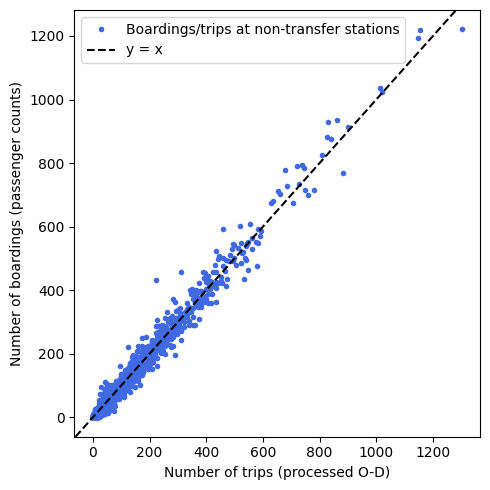
\includegraphics[width=0.5\linewidth]{images/Validation/inputvsdatavic.png}
    \caption[Comparison between input O-D and passenger counts data at non-transfer stations]{Comparison between input O-D and passenger counts data at non-transfer stations with a linear line of best fit.}
    \label{fig:inputvsdatavic}
\end{figure}
\subsubsection{Comparing functions and coefficients }
Using the four different crowding cost functions built into WoB, the model outputs could then be compared to identify the impact of these crowding cost functions. Since each function represents a different relationship between the number of passengers and crowding cost, there should be an observable difference in the trip choices made by the simulation agents. The same process was undertaken as for comparing the input O-D to the passenger counts data, wherein the model output was plotted on the x-axis and the passenger counts data on the y-axis, for each hour at each non-transfer station. The closeness of the linear fit to the line $y=x$ and the absolute difference between the datasets was used to assess the best crowding cost function for the case study. 

To ensure consistency between the functions, the same parameters and capacity values were used ($\alpha_0=0.25, \alpha_1=0.5, a=5, b=1, c=0.01$). The linear crowding cost function output had the best fit, producing a slope of $0.95$ with an absolute difference of $41,211.51$, the quadratic function had a slope of $0.94$, while both the one- and two-step models produced a slope of $0.93$. The full plots for all four functions can be viewed in Appendix II. However, to determine whether varying the parameters for the one- and two-step would improve how well the model output fits to the passenger counts data, a combination of different parameter values were also tested. 

The full table of parameters tested and the fit results (including the slope and standard deviation) is available in Appendix II. Out of the combinations tested, the two-step model performed the best with a slope of $0.96$ and an absolute difference of $37,341.33$ with the parameters $\alpha_0=0.25, \alpha_1=0.5, a=5, b=0.5, c=0.02$ (\Cref{fig:two_step_final}). This difference between the model output with the two-step crowding cost function and the passenger counts is within the margin of error due to the difference between the input O-D data and the passenger counts. Therefore, the two-step crowding cost function with the aforementioned parameters was used for the case study data analysis. 

\begin{figure}
    \centering
    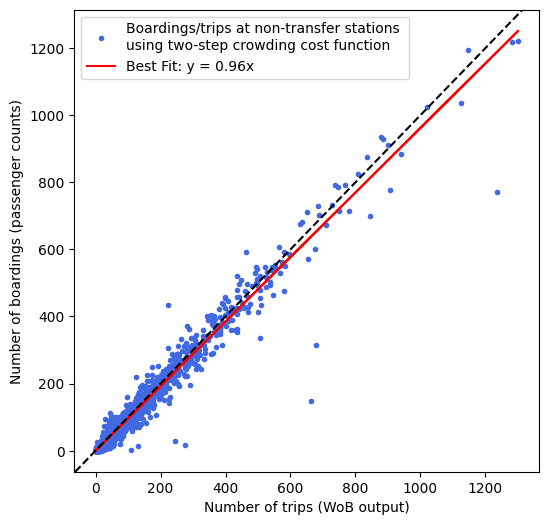
\includegraphics[width=0.5\linewidth]{images/Validation/two_step_final.png}
    \caption[Comparison between WoB journey output and passenger counts data at non-transfer stations]{Comparison between WoB journey output and passenger counts data at non-transfer stations with a linear line of best fit.}
    \label{fig:two_step_final}
\end{figure}

\section{Methodology}
\label{sec:methodology}
The network was generated using a GTFS file spanning from September 6th to December 8th. The modelled date was set to September 9th, 2024, a normal Monday. There were no major planned disruptions due to the ongoing Victorian Big Build works, but there were some overnight closures. %( CITE https://mobilitydatabase.org/feeds/mdb-657 and https://bigbuild.vic.gov.au/disruptions/calendar) 
The processed O-D was used as input patronage information, and trip capacities were supplied to specify the varied train capacities for each train line, as described in \refandname{sec:data}. The two-step crowding cost function was used, as justified in \refandname{subsec:validation_crowding}. Three rounds were modelled as the model converges on a stable solution at this point (\Cref{subsec:convergence}). 

\subsection{Network Utilisation}
% Max count map
In order to visualise spatial peak rail network utilisation, the maximum counts for each pair of adjacent stations (connections) was found for the morning peak period (7am-10am) using the WoB agent counts output. Adjacency was defined by trips, not by spatial proximity, so express service connections bypass some stations. The connections were colour coded according to the value of the maximum passenger count and plotted on a map. 

% Network utilisation graph
To visualise temporal network utilisation, the agent count data needed to be re-indexed on a per-minute basis, rather than as a list of variable periods of time. To this end, an array indexed by each minute of the day was initialised to zero, and for each connection record in the agent count output the departure and arrival time of each connection was added to the relevant segment of the indexed array. This array then encoded the total network utilisation during each minute of the day.

\subsection{Sustained Crowding}
% Number of services w/ sustained crowding (text/ wordy stuff)
Sustained crowding was investigated by analysing the number of connections per trip, that exceeded the seated capacity. Using the WoB agent counts output, these connections were summed and divided by the total number of connections in that trip to determine the proportion of total trips which were above seated capacity. 

% Standing Hours
To calculate the number of hours spent standing on trains throughout the day, the duration of each connection in minutes was multiplied by the number of standing agents (the total agent count minus the seating capacity, with a minimum value of zero) to determine the per-connection standing minutes. Then, connections were grouped by train line and the standing minutes summed together, after which the standing minutes were converted to hours.

\subsection{Timetable Modification}
% Timetable editing and loading
To demonstrate WoB's ability to assess the impact of timetable changes, a modified GTFS file was used to produce a comparison of passenger loads when a service was added. The service with the highest passenger count was chosen, as it was expected that an additional service would help alleviate crowding and produce a change in passenger loads. This was found to be the 7:23am in-bound Cranbourne service. This trip was duplicated and given a new trip ID in the GTFS file and the stop times were delayed by 2 minutes, producing a new 7:25am in-bound Cranbourne service. The trip capacities file was also updated with the new trip ID and the same train capacity as the original 7:23am service. Two plots of passenger loads across the stations were produced, one without the additional service and one with it, to observe the impact of the new service. The services immediately before and after the 7:23am service (at 7:11am and 7:38am) were also included to observe any shifts in passenger loads. 

\subsection{Transfers}
Transfers were defined by journeys that involved boarding more than one service. The number of transfers taken per station was quantified by summing the number of agents per station from the transfers output from WoB. The stations were then colour coded according to the number of transferring passengers and plotted on a map. 

\subsubsection{Journey Types}
\begin{figure}[ht]
    \centering
    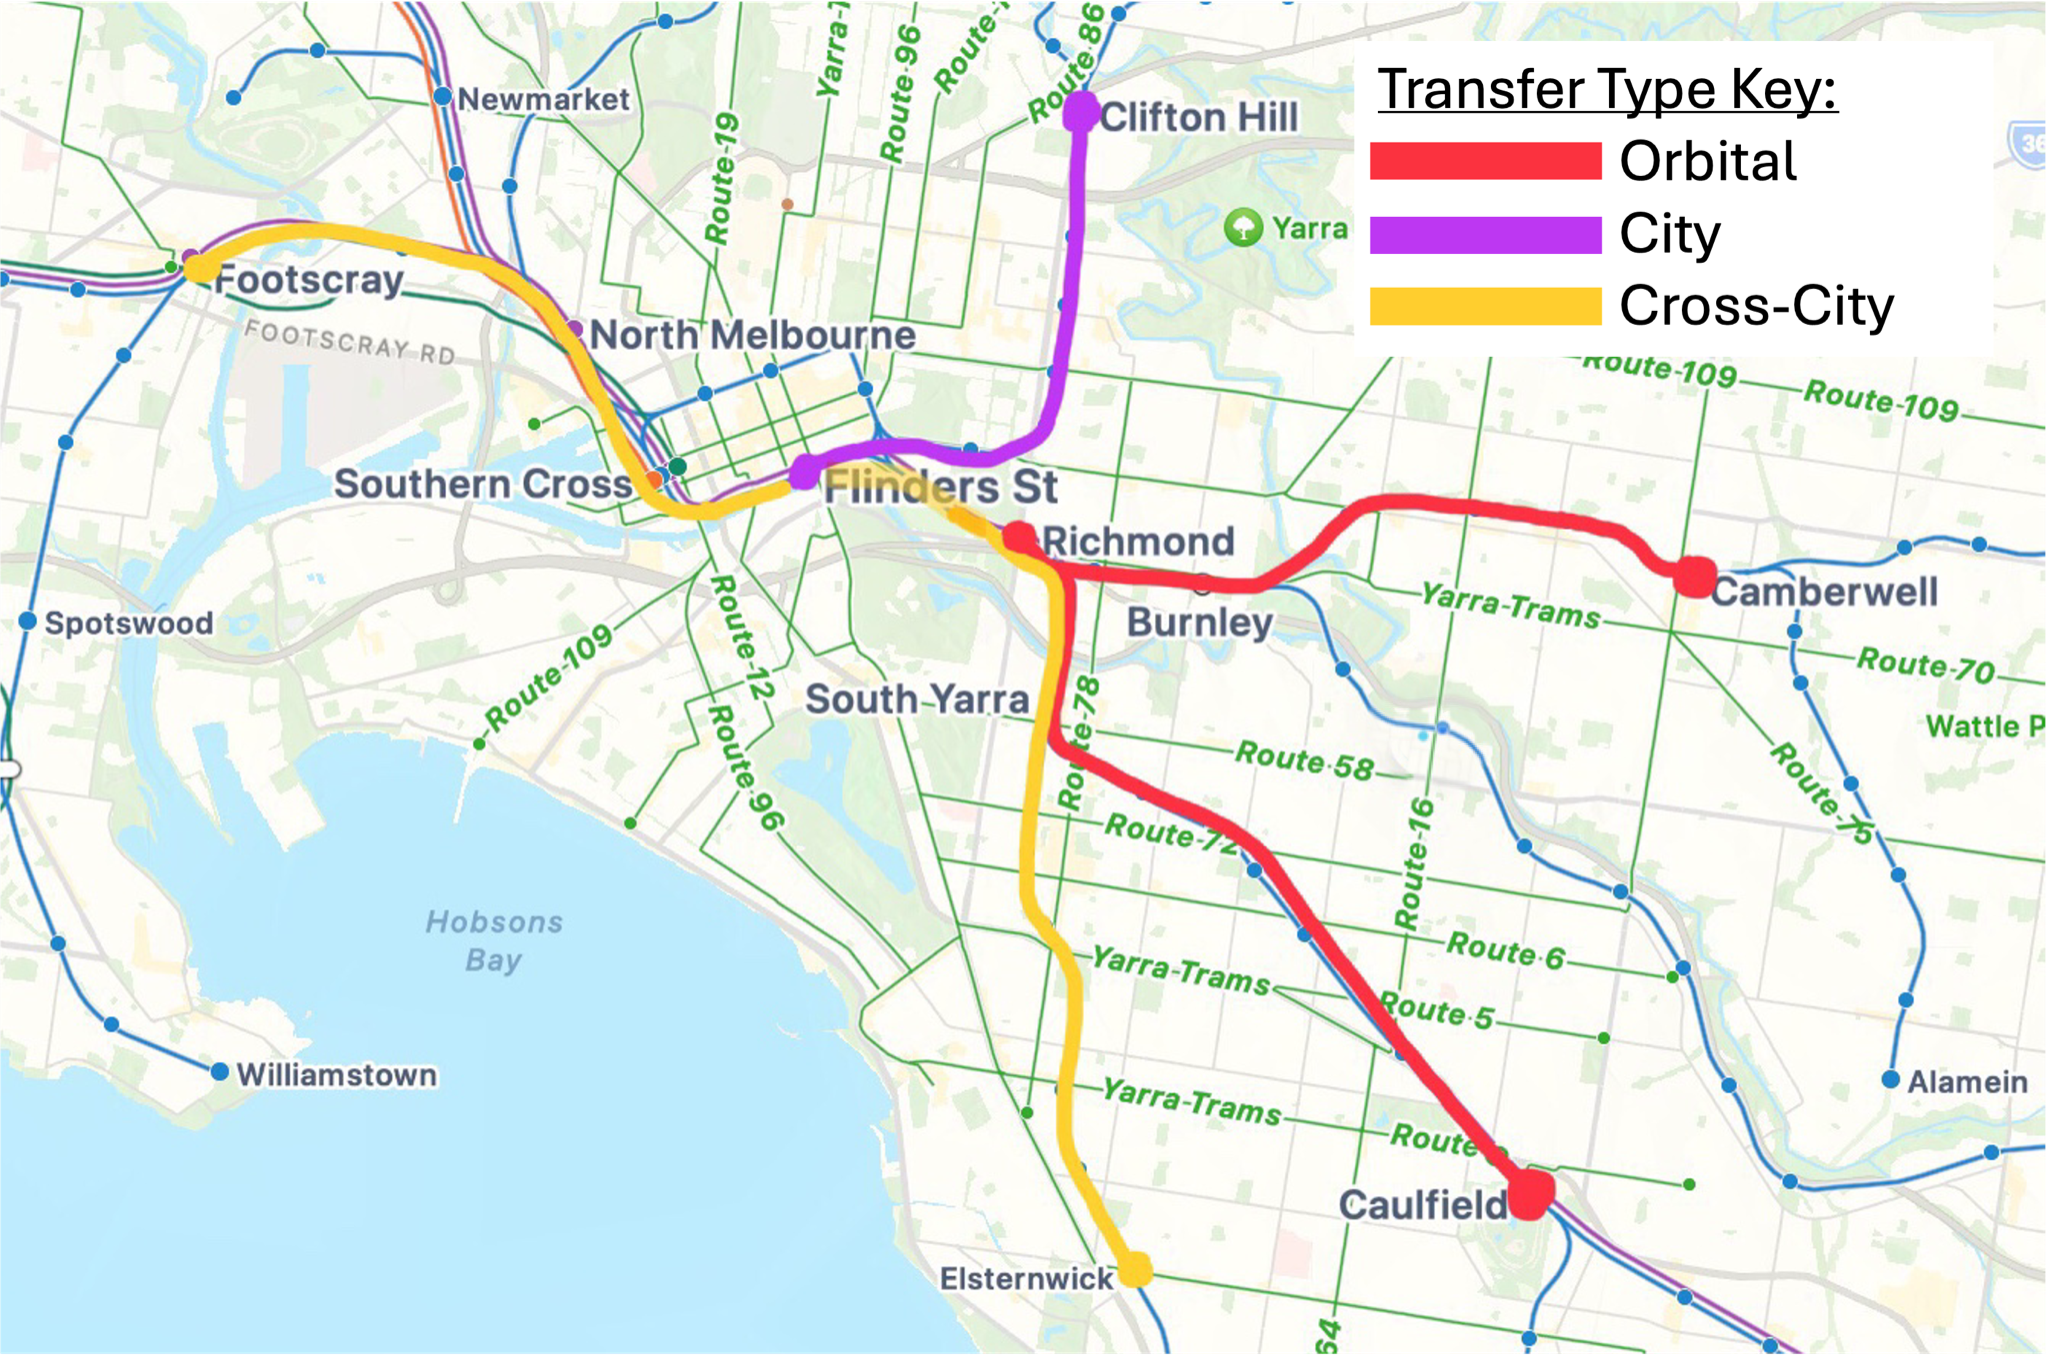
\includegraphics[width=0.75\linewidth]{images/Case_Study/diagram_assigning_groups_transfers.PNG}
    \caption{Example journeys that demonstrate orbital, cross-city or city characteristics. }
    \label{fig:transfer-diagram}
\end{figure}
Using the WoB journeys and legs output, trips with at least one transfer were assigned into three main categories: city, cross-city or orbital. \Cref{fig:transfer-diagram} illustrates example journeys for each of these categories. City trips were defined as trips starting or ending in the CBD (City Loop stations), or nearby major stations such as Richmond, Jolimont, South Yarra and North Melbourne, as demonstrated by the purple line. Orbital trips are trips where the origin-destination points are orbital, but due to the radial network layout involve extra travel to transfer at a common junction station. An example of this is shown in red in \Cref{fig:transfer-diagram}, where travel between Caulfield and Camberwell involves extra travel into Richmond Station to interchange. Cross-city trips occur when the journey involves crossing through the city, as demonstrated by the yellow trip connecting Elsternwick and Footscray. To differentiate between orbital transfers and cross-city transfers, the lines were grouped and rules were assigned to determine cross-city or orbital relationship. The precise assignment process is outlined in Appendix III.

To investigate where the travellers making transfers were coming from and heading to, stations in the network were classified as being "inner" or "outer", based on whether they were reachable within 20 minutes from Flinders Street Station. Journeys beginning and ending in different zones were assigned as "inner and outer". Of the journey types (orbital, city, cross-city), the number of agent taking journeys across the different zones was summed. 

\subsubsection{Platform Transfers}
Platform transfers at Flagstaff, Melbourne Central and Parliament were visualised by filtering the agent transfers WoB output for transfers occurring at these stations. These three stations have fixed platforms for each train group, which are the same for all three stations and are specified in Appendix III. The volume of agents making transfers between each of the four platforms was plotted on a matrix. 

\section{Results and Discussion}
\label{sec:resultsanddiscussion}
\subsection{Network Utilisation}
\begin{figure}[ht]
    \centering
    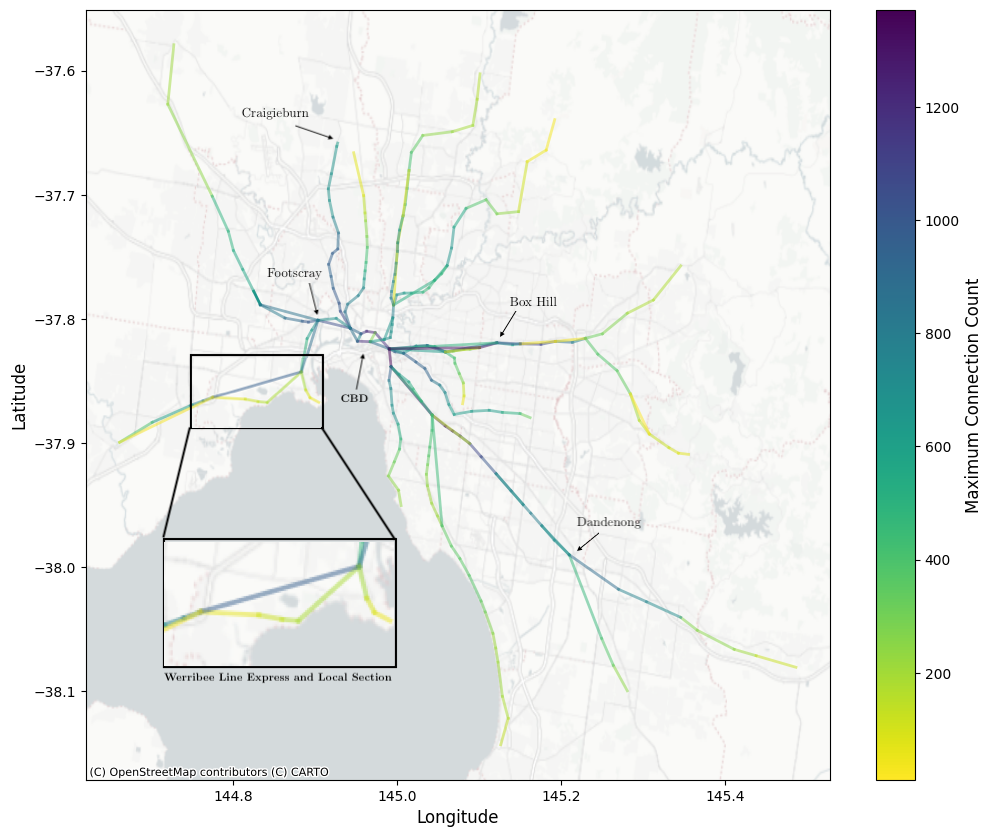
\includegraphics[width=\linewidth]{images/Case_Study/max_count_map_labelled.png}
    \caption[Maximum connection passenger count]{Maximum passenger count between each pair of subsequent stations during the morning peak period (7am-10am). The Werribee express service has been magnified.}
    \label{fig:max_connection_map}
\end{figure}
\Cref{fig:max_connection_map} shows the maximum passenger count between each pair of subsequent stations (connections) in the morning peak period (7am-10am). This includes express services overlaid as these often have high patronage during peak times. The Werribee express has been magnified on the map, showing the higher maximum passenger count, compared to the stopping all stations via Altona service. A network schematic map is available in Appendix III. The corridor between the CBD and Dandenong, Craigieburn, Box Hill and Footscray all have high maximum counts. The patronage towards the ends of lines tend to be lower than the middle to inner regions of the lines. 

Due to the radial nature of the metropolitan rail network and the high density of workplaces in the CBD, majority of train use during the morning peak is into the CBD. \Cref{fig:max_connection_map} shows the expected trends with the maximum number of passengers through connections increasing towards the inner city. While station pairs around the City Loop have the highest sum of passengers travelling through them, the high frequency of services means that the maximum count on a single service is lower than some of the other inner city connections such as from Richmond to Parliament. WoB's agent count output enables the quantification of these patterns, to understand which connections are highly utilised at different times. \Cref{fig:max_connection_map} also shows express connections such as the Werribee line express via the bypass, which has a higher maximum patronage than the individual connections through the stopping all stations Altona loop section. Understanding how these express services are utilised differently enables more nuanced provisioning of these services. 

\begin{figure}[ht]
    \centering
    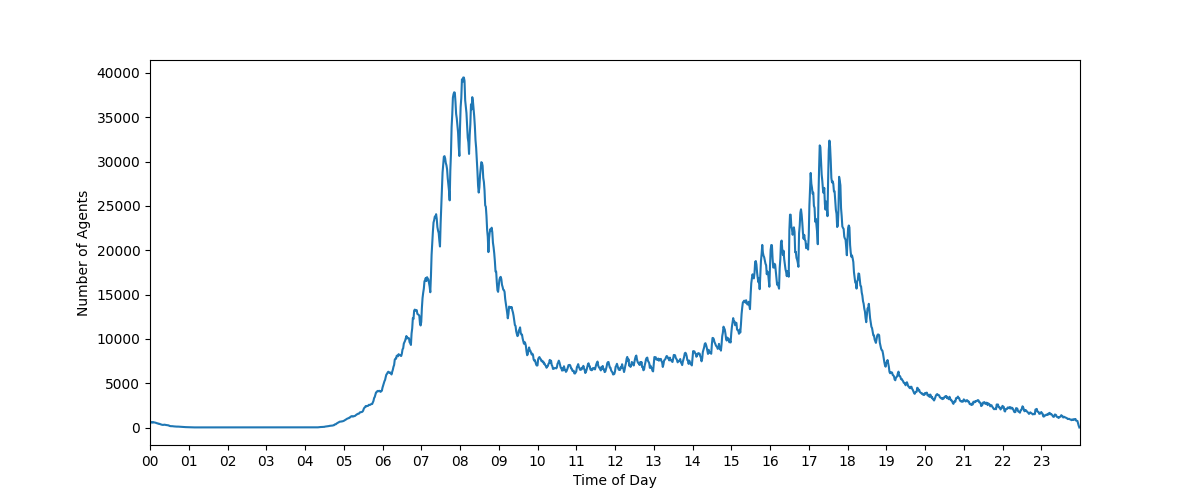
\includegraphics[width=\linewidth]{images/Case_Study/network_util.png}
    \caption[Network-wide utilisation]{Minute-by-minute network-wide utilisation. }
    \label{fig:network_utilisation}
\end{figure}

% RESULTS
Figure \ref{fig:network_utilisation} shows the agent count per minute across the entire network. This provides insight into the number of people aboard trains at any given time, allowing the busiest windows to be observed. A high morning peak is observed between 7am-9am, and a lower yet longer afternoon peak occurs between 3pm-6pm. 

The two peaks in network utilisation occur during the expected peak period ranges. The AM peak period sees a higher volume of people over a shorter time window than the PM peak period, which tends to be elongated on weekdays due to the staggered finishing times of school and work. This was observed in semester one work on peak periods for train usage \cite{tranChangesPeakPeriods2024}.

While \Cref{fig:network_utilisation} provides a snapshot of the number of people on services at a network-wide level, it can also be specified to a particular train station or region, demonstrating the granularity possible when using WoB. There are a range of applications in which this can be utilised, including understanding the time between each of the peaks and the length of the peaks. This can provide useful context when making decisions on station dwell times and transfer timings in timetable evaluation. 

The periodic spikes observed in \Cref{fig:network_utilisation} is due to the binning of the input data by 15 minute intervals, as described in \refandname{sec:data}. As agents start their journey at the beginning of a 15 minute block, they begin boarding trips immediately, leading to a spike in the number of agents in the network. However, no new agents enter the system for the remainder of that 15 minute block, so the only effect on the system is agents arriving at their destination and being removed from the network, leading to an overall drop in utilisation. More detailed O-D data would allow agents to be generated more naturally to prevent this type of artefact. 

\subsection{Sustained Crowding}
In order to gain a more comprehensive understanding of crowding, the levels of sustained crowding on train services was measured as the proportion of stops for which a service was above seated capacity. 93\% of services were found to be above seated capacity for less than 10\% of the total stops on a given trip.

Only 36 out of 2,592 services exceeded seated capacity for over half of the stops in the total trip. The Alamein, Frankston, Upfield, Williamstown and Belgrave lines did not have any trips with crowding above seated level for half of the trip. The Werribee and Hurstbridge lines had the greatest number of trips which were occupied to this extent, with 8 and 6 respectively, all of which occurred within the AM (7am-10am) and PM (3pm-6pm) peak periods. 

% describe results for passenger hours
Crowding can also be quantified by measuring the total number of hours for which passengers on each line are required to stand (\Cref{fig:standing-minutes}). The Belgrave, Craigieburn, Sunbury and Werribee lines all had high numbers of passenger hours spent standing. The Alamein, Frankston, Upfield, Sandringham and Williamstown lines were comparatively very low. 

\begin{figure}[ht]
    \centering
    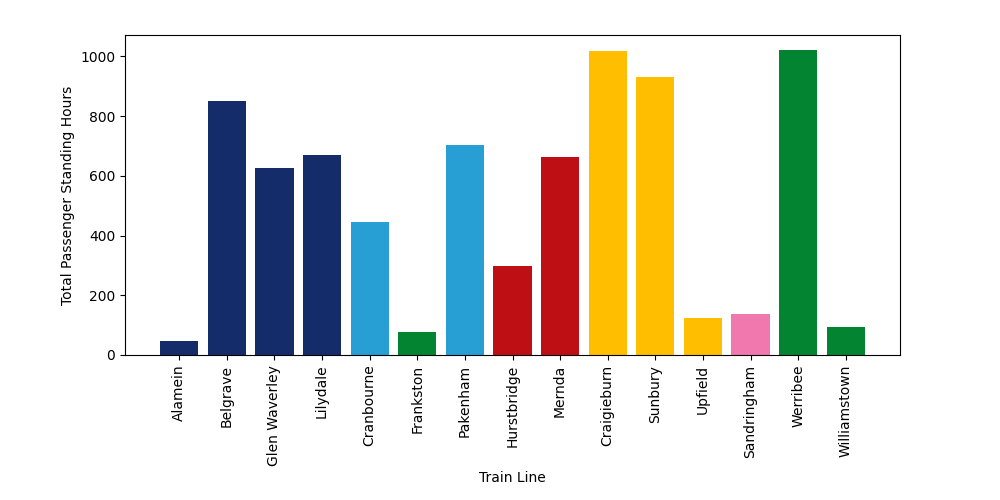
\includegraphics[width=0.85\linewidth]{images/Case_Study/standing_hours.png}
    \caption[Hours passengers spent standing over a single day]{The total amount of time passengers spent standing over a single day for each train line of the network. The colours are defined by the GTFS route colour, which matches their colour on passenger-facing information displays.}
    \label{fig:standing-minutes}
\end{figure}

Given the highly radial train system serves some regions with relatively small population catchments (e.g. Hurstbridge and Tecoma), it was expected that many services would experience crowding in the inner city regions. Longer train lines such as Belgrave and Frankston did not have any trips above seated capacity for more than half of the journey length, which is consistent with the lower agent counts in the outer connections observed in \Cref{fig:max_connection_map}. Craigieburn was found to have consistently high passenger hours standing and maximum agent counts for majority of the trip connections during the AM peak period. 

Quantifying passenger time spent standing provides a passenger-focused method for evaluating public transport service changes. This metric can provide greater insights for how service changes impact passenger comfort. The Belgrave line has a relatively high amount of standing time, given there were no services with crowding above seated capacity for over half the stops. Combining these two crowding metrics suggests that the Belgrave line is more likely to experience shorter periods of intense crowding which contributes to the large quantity of passenger standing time. Conversely, Craigieburn has a high amount of standing time but also has four services above seated capacity and high maximum connection counts. This suggests that Craigieburn experiences sustained crowding across the line. These examples highlight the ability of WoB to produce novel outputs that can be combined to illustrate a nuanced picture of the transport network. 

The standing time calculation assumes that people only stand once all seats have been filled. While this is possible on the HCMT trains with open corridor connections, all other train models would require a passenger to change carriage at a station to access seats on other carriages. 

\subsection{Timetable Modification}
\begin{figure}[ht]
    \centering
    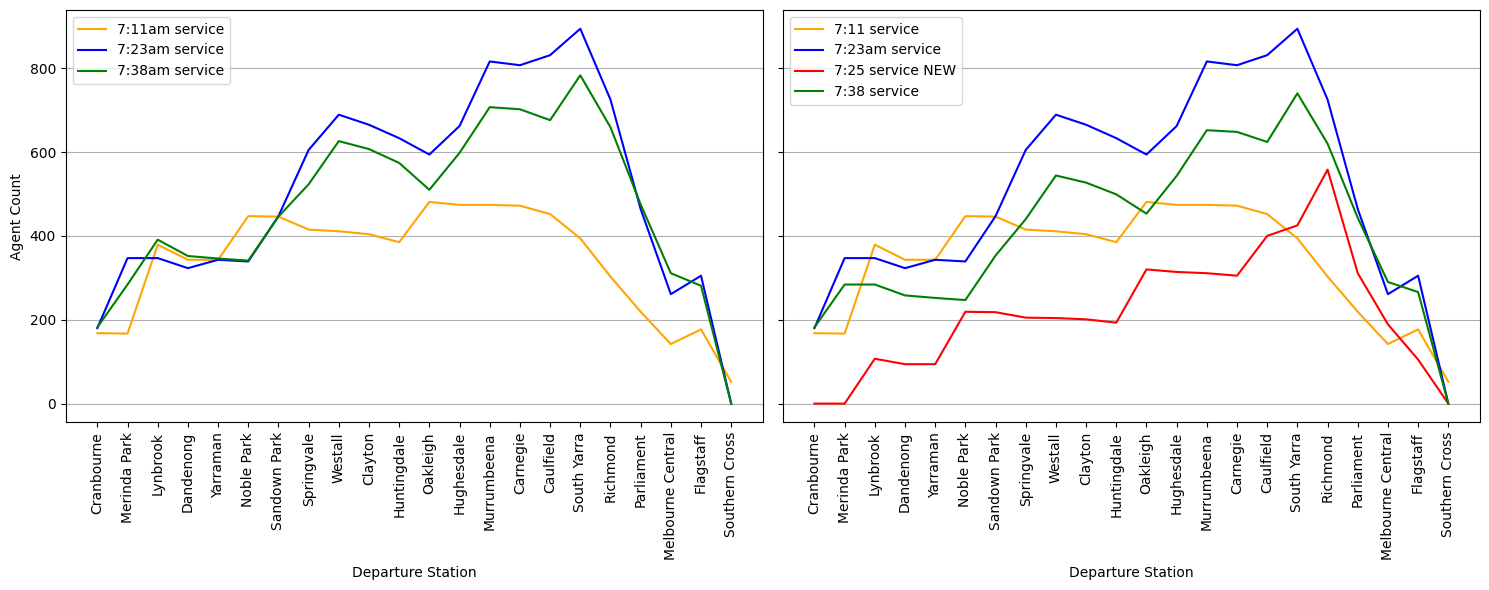
\includegraphics[width=1\linewidth]{images/Case_Study/gtfs_edit.png}
    \caption[Passenger counts between connections aboard in-bound AM peak Cranbourne services, with the addition of a new service]{Passenger counts aboard in-bound AM peak Cranbourne services, with the addition of a new service. (Left) Services in the original timetable. (Right) Services with a 7:25am service added. As passenger counts are measured between station connection pairs, the stations listed on axis are the departure stations.}
    \label{fig:CBE_add_service}
\end{figure}

Figure \ref{fig:CBE_add_service} shows the results of an altered timetable, where an additional in-bound Cranbourne service was added at 7:25am, 2 minutes after the existing 7:23am service. This demonstrates how WoB redistributes passengers when the timetable is changed. All three of the existing services show similar shapes of patronage across the stops before and after addition of the new service. The redistribution of demand to the new service is apparent in the reduction in patronage on the 7:38am service. 

The drop in patronage on the 7:38am service as a result of the additional 7:25am service in \Cref{fig:CBE_add_service} shows agents have decided to take the earlier and less crowded 7:25am service. The changes observed across these figures highlights agent journey replanning by WoB, and demonstrates how network utilisation changes in response to service changes. 

In the scenario with the additional service, there are 4,773 people on board the new 7:25am service while the 7:38am services has 1,180 fewer passengers. Both the 7:11am and the 7:23am show no changes in patronage as a result of the new service. The fact that the total patronage in the new service scenario is greater than that of the original timetable indicates that passengers previously taking services on other lines have made transfers to the Cranbourne line to avoid crowding. Prior to Dandenong, which is the first station with transfer opportunities, the total patronage on the four services in the new service scenario is the same as the original three services. This shows that when transfers are not possible, the change in patronage is entirely due to people choosing the new 7:25am service over the 7:38am service. 

This example shows how WoB can be used to evaluate timetable changes by quantifying their impact. Although quantifying the effect of timetable changes by hand is challenging due to the multitude of factors influencing decision-making, WoB's simulation provides a foundation for modelling this decision making.

The current version of WoB does not feature built-in GTFS modification tools, requiring the GTFS files to be manually edited to include the additional service. Whilst WoB can handle evaluating more widespread timetable changes, the workflow to achieve this is currently limited by laborious manual GTFS manipulation. A key feature to increase the speed of timetable evaluation workflows in WoB would be an inbuilt interface for GTFS modification. This would support faster iteration of different timetable scenarios for applications such as transport planning and consultation. 

\subsection{Transfers}
WoB's ability to match origin-destination station pairs to network-based journey itineraries provides greater detail into how users make transfers. This enables deeper exploration of demand at and within stations by revealing where transfers are made, as opposed to just the station entry and exit volumes. As 43.4\% of all journeys involve making a transfer and current data does not adequately capture the details of this behaviour, WoB was used to further investigate transfer patterns. 

\begin{figure}[ht]
    \centering
    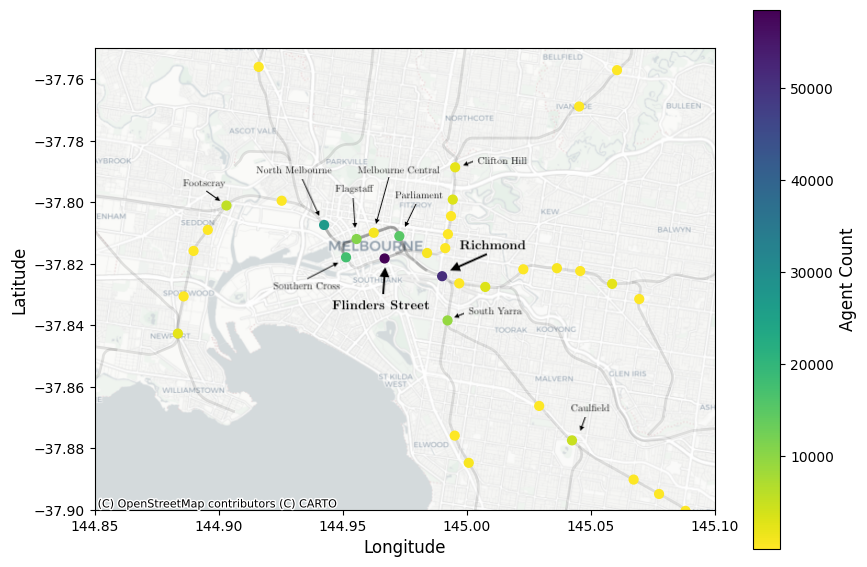
\includegraphics[width=1\linewidth]{images/Case_Study/transfer_map_labelled.png}
    \caption{Number of agents making transfers at stations, colour coded by volume of agents.}
    \label{fig:transfer-map}
\end{figure}

\Cref{fig:transfer-map} visualises the number of transfers made by agents at stations over a normal Monday. Flinders Street and Richmond Station exhibited the highest number of transfers, followed by North Melbourne, Southern Cross, Parliament, Flagstaff and South Yarra Station. Further from the CBD, a moderate number of transfers are also made at Footscray, Caulfield, Burnley and Clifton Hill. Of journeys made which included a transfer, 69\% of these started or ended at CBD stations. 13\% were cross-city and 18\% were orbital. 


% tie the map into the following statistics - at those transfer stations, the purpose of people's transfers were investigated. 64.2\% of agents made trips which started or ended at the CBD stations. Of the remaining agents, 23,587 made cross-city trips, and 33,402 took journeys that we classed as orbital. 

\begin{figure}[ht]
    \centering
    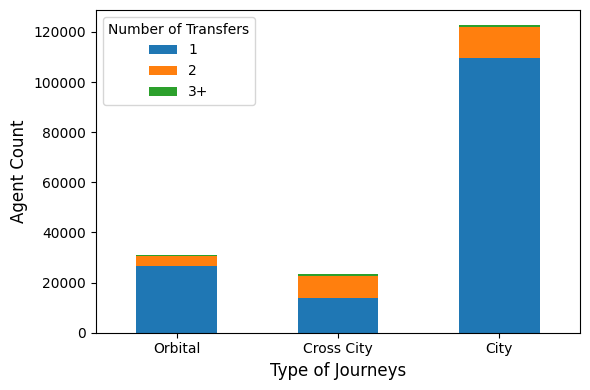
\includegraphics[width=0.75\linewidth]{images/Case_Study/journeytypetransfers.png}
    \caption{The number of agents making different types of journeys and the number of required transfers for those journeys.}
    \label{fig:transfers_type}
\end{figure}
% RESULTS
Figure \ref{fig:transfers_type} highlights the number of transfers taken within each trip type for all trips involving a transfer. City trips are by far the most popular trip type, making up 69\% of all trips with transfers. Despite cross-city trips being less commonly taken, a greater proportion of them require at least two transfers, compared to orbital trips which are largely made with a single transfer. 

To investigate where the travellers making transfers were coming from and heading to, stations in the network were classified as being "inner" or "outer", based on whether they were reachable within 20 minutes from Flinders Street Station. 70\% of journeys involving transfers were found to end in the city. For agents starting or ending in the city, 17\% travelled only within inner regions, while the remaining 83\% covering both inner and outer. For cross-city trips, 50\% covered both regions, while 42\% were in outer regions, and only 8\% were in inner only. Orbital trips exhibited a similar split, with 55\% in both regions, 39\% in outer regions, and only 6\% were inner only. 

\begin{figure}[ht]
    \centering
    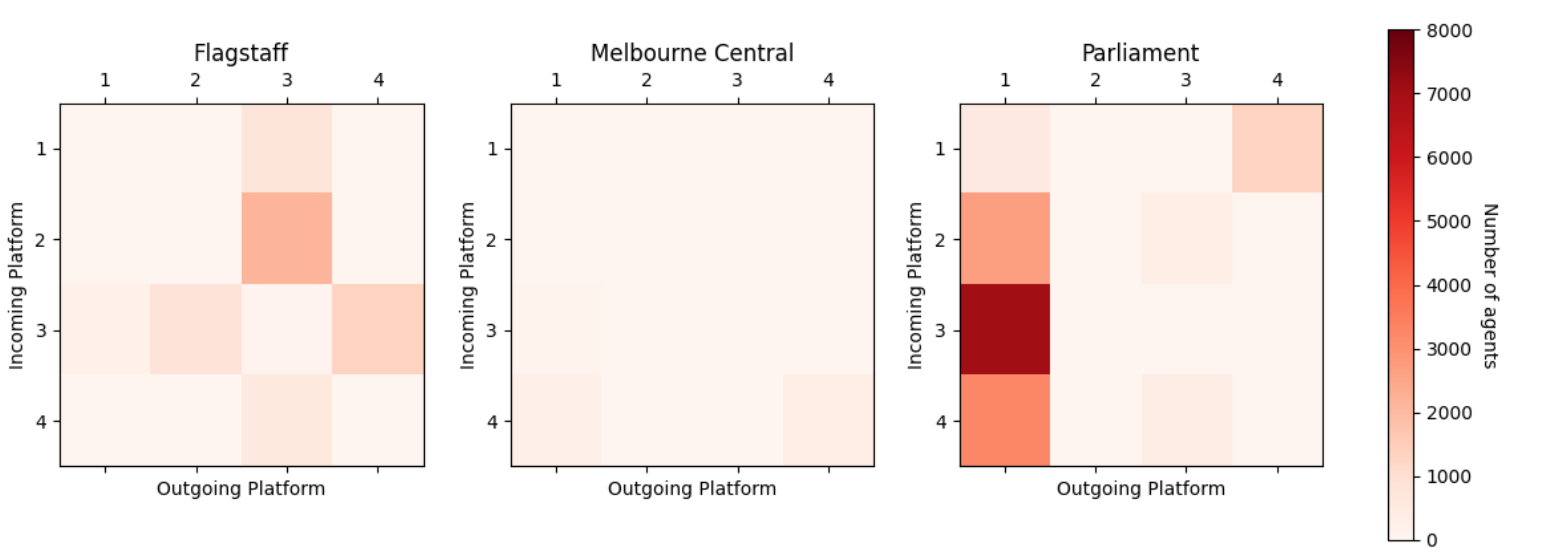
\includegraphics[width=1\linewidth]{images/Case_Study/city_loop_platform_transfers_geog.png}
    \caption{A matrix representation of the number of transfers that occur between the 4 platforms of the City Loop stations with fixed platforms for different train groups}
    \label{fig:platform_matrix}
\end{figure}

% RESULTS - CITY LOOPS
\pagebreak{}
To understand transfer behaviour and the implications for timetabling and station planning, platform transfer patterns were visualised in \Cref{fig:platform_matrix} for the CBD City Loop stations with fixed platforms for different train groups (as assigned in Appendix III). At Parliament, most transfers involved Platform 1, with the greatest number of agents transferring from Platform 3 to Platform 1. At Melbourne Central, there were fewer transfers and no clear trends. At Flagstaff, the greatest number of agents transferred from Platform 2 to Platform 3. 

% DISCUSS TRANSFER MAP
The results of both \Cref{fig:transfer-map} and \Cref{fig:platform_matrix} highlights that very few transfers are modelled for Melbourne Central Station. In the City Loop, Melbourne Central is between Flagstaff and Parliament, so the majority of optimal journey itineraries will prefer either Flagstaff or Parliament. The RAPTOR algorithm will always choose the earliest transfer opportunity in order to maximise available transfer time, which preferences Flagstaff and Parliament over Melbourne Central. However, actual passengers are unlikely to exhibit this extreme rationality for the most optimal travel route and instead tend to have personal preferences for different City Loop stations. % cite transfer dislike or preferences of certain places

% discuss number of transfers per journey type 
The high number of journeys starting or ending in the city in \Cref{fig:transfers_type} is likely due to the radial nature of the network. Orbital trips cover larger distances and take longer, and are therefore less time efficient than driving. However, there is still demand for orbital and cross-city trips. Orbital trips are largely completed with only one transfer, likely due to the limited options for transferring at outer stations. Melbourne's prospective Surburban Rail Loop project caters to these orbital trips, and would generally involve two transfers but provide a faster trip, as it doesn't require passengers to travel to the inner city before making a line transfer. 

Transfer behaviour cannot be measured from O-D data or patronage volume information alone, and requires modelling of these datasets to interrogate. As transfer opportunities on the Melbourne train network become increasingly complex with the opening of the Melbourne Metro Tunnel and the prospective Suburban Rail Loop project, understanding transfer behaviours is essential to inform network and station design decisions. The impacts of different network configuration scenarios can be measured at the micro and macro scale. Network-wide impacts on station transfer volumes can be visualised as in \Cref{fig:transfer-map}. At a station level, platform transfer matrices such as \Cref{fig:platform_matrix} can provide further details of how these transfer volumes between different platforms change. 

\section{Limitations}
\subsection{Input Data}
The robustness of results found in the case study is limited by the input data and processing choices. The input O-D and passenger counts data were found to be similar but not identical, limiting the validation process for the model output. The uncertainty surrounding the accuracy of the input data also limits the exact conclusions which can be drawn from these findings. However, they are likely indicative of broad trends and demonstrate WoB's capabilities for these use cases. 

The two DTP datasets used, the input O-D and passenger counts data, were processed using TrainSUM to impute missing or unpaired trips. The rate of missing or unpaired trips TrainSUM had to impute was not stated. TrainSUM models journeys with at most 1 transfer, compared to WoB which allows up to 7, suggesting that these models will behave quite differently \cite{victoriandepartmentoftransportandplanningAnnualMetropolitanRegional2024}. However, the specific algorithms used by TrainSUM are unknown and therefore the implications of this processing on the datasets is unclear. Therefore, all the data used in this project was influenced by TrainSUM's processing, and ideally in future work, access to the actual raw O-D data would improve the handling of transfers. 

Only a single normal Monday was modelled, which may not capture the nuances of variation in service demand across weekdays. Work completed in semester one found that the 2022-2023 financial year had lower patronage on Mondays and Fridays which would likely extend into the 2023-2024 financial year, due to the ongoing impact of changes to working from home patterns after the COVID-19 pandemic \cite{tranChangesPeakPeriods2024}. This limited the generalisability of these results, but provided a snapshot of the current period. 

While the accuracy of the drawn results and conclusions was bounded by the limitations of the input data, this was not central to the project's aim of building a model that processes O-D data to quantify service level utilisation. Therefore, the results presented here are not intended to be an exhaustive measure of rail utilisation in Melbourne, but instead highlight the potential of WoB for transport modelling. 

\subsection{Disruptions}
Since the input O-D data is aggregated across each financial year, the impacts of scheduled disruptions cannot be accounted for. If there were extended periods of time with buses replacing trains, there would be lower demand recorded for those services, which, when applied to a normal timetable, would appear as if services were not particularly crowded. In actuality, some demand may have been suppressed due to the unavailability of the usual train services. Conversely, normal patronage demand data applied to a disrupted train schedule GTFS with reduced services, would assign a larger volume of people to fewer services, unrealistically increasing crowding. While September 9th, 2024 was chosen for this case study as there were no major planned disruptions due to Big Build works, there were still some disruptions in the evening. There is no definitive centralised source of public information on disruptions so there was no way to determine the confounding effects of these factors.

Unplanned disruptions or delays are also not accounted for as WoB uses the planned timetable and not real-time vehicle movements. The assignment of journeys from smart card data to services may not reflect real journeys taken. The ability to account for cancellations or delays would enable more accurate measures of crowding as these events would shift demand to other services. 


\subsection{Station Transfer Modelling}
An additional limitation of the current setup of the model is the accuracy of how transfers are modelled. The minimum allowable transfer time was set to three minutes for all agents at all stations. WoB will not consider any trips where the next leg of the trip begins less than three minutes after the initial arrival time. However, depending on station layout and walking speed, there are multiple opportunities for cross-platform transfers which take less than three minutes. Further research into transfer behaviour would inform a more precise model of how transfers occur in the Melbourne network. 


\chapter{Future Work and Conclusion}
\label{chap:Conclusion}
\section{Future Work}

\section{Conclusion}


\backmatter
\pagenumbering{roman}
\appendix
\chapter{Appendix I: Glossary}
\centering
\DefTblrTemplate{caption}{default}{}
\DefTblrTemplate{middlehead,lasthead}{default}{}
\begin{longtblr}[caption={Glossary},entry=none]{colspec={l|X}, rowhead=1}
    Term     & Definition                                                                                                         \\ \hline
    Agent    & An entity with agency (i.e. decision-making capability). Often used in terms of a simulation that individually models discrete states. \\
    BRT      & Bus Rapid Transit.
    A high frequency bus network with sections of exclusive right-of-way and priority at intersections.                           \\
    CSA      & Connection Scanning Algorithm. Timetabled pathfinding algorithm.                                                   \\
    Dijkstra & Dijkstra's pathfinding algorithm.                                                                                  \\
    DTP      & Department of Transport and Planning (Victorian Government Department).                                            \\
    GTFS     & General Transit Feed Specification. A standard for specifying public transport systems.                            \\
    MATSim   & Multi-Agent Transport Simulation. An extensible open-source simulator for agent-based microsimulations.            \\
    MC       & Multi-criteria (pathfinding problem extension).                                                                    \\
    RAPTOR   & Round bAsed Public Transit Optimised Router. Timetabled pathfinding algorithm.                                     \\
    TD       & Time-dependent.
    Used to refer to a graph representation of a timetabled network where each edge has a weight dependent on the departure time. \\
    TE       & Time-expanded.
    Used to refer to a graph representation of a timetabled network where each timetable stop is a separate node.                 \\
    VITM     & Victorian Integrated Transport Model.
    The comprehensive transport model used by the DTP to forecast travel demand across Victoria.                                  \\
\end{longtblr}


\printbibliography[title=References]
\end{document}
